\documentclass{article}
\usepackage{lmodern}
\renewcommand{\rmdefault}{lmss}
\usepackage[T1]{fontenc}
\usepackage[utf8]{inputenc}
\usepackage{float}
\usepackage{graphicx}
\usepackage[margin=1in]{geometry}
\usepackage{titlesec}
\usepackage{inconsolata}
\usepackage{hyperref}
\usepackage{subcaption}
\usepackage{amsmath}
\usepackage{amssymb}
\usepackage{mathtools}
\usepackage{indentfirst}
\newcommand{\code}[1]{{\fontfamily{zi4} \selectfont{#1}}}
\newcommand{\sectionbreak}{\clearpage}
\setcounter{secnumdepth}{2}
\usepackage{fancyhdr}
\pagestyle{fancy}
\fancyhf{}
\fancyhead[L]{\leftmark}
\fancyhead[R]{\thepage}
\renewcommand{\headrulewidth}{0.4pt}
\DeclarePairedDelimiter\floor{\lfloor}{\rfloor}
\hypersetup{colorlinks=true, urlcolor=cyan, linkcolor=[rgb]{0.05,0.05,0.05}}

\begin{document}

\begin{titlepage}
   \begin{center}
   
       \vspace*{7cm}

       \huge{\textbf{Machine Learning}}
          
       \vspace{0.5cm}

       \Large{Shanmugha Balan S V}
       
       \vspace{4.5cm}
       
   \end{center}
\end{titlepage}

\tableofcontents

\section*{Preface}
These are the notes I made while learning machine learning. The information has been taken from various sources. Some of the major contributing sources were the \href{https://scikit-learn.org/stable/modules/classes.html}{API of scikit-learn}, the \href{https://www.coursera.org/learn/python-machine-learning}{Applied Machine Learning course} by University of Michigan.

Most of the images were generated with code which can be found in this \href{https://github.com/sbalan7/ML-and-Stats}{repository}. In case you'd like to contribute to this by adding more information, or you find any error at any position in the text, please open a pull request for the repository above. It also has the LaTeX file for this document. If you want a permalink to the pdf, please use this \href{https://github.com/sbalan7/ML-and-Stats/tree/master/LaTeX Notes/machine_learning.pdf}{link}.

Version 5.2
January 2021

\section{Machine Learning - Basics}

\subsection{Types of Learning}

Machine Learning is broadly split into supervised learning and unsupervised learning. In supervised learning, we make the model fit to input-output pairs, so when the model is fed in with new data, it gives a similar output. The outputs are labelled in supervised learning. In unsupervised learning, the module makes arbitrary divisions, with no labelling of data. It finds clusters of similarities in the data presented to it.

Supervised learning methods mainly fall into two subcategories - classification and regression. In a classification problem, data is presented as belonging to a labelled group. It has discrete categories. Classification can be binary or multi class. Binary classification is between two groups - a positive class and a negative class. Multi class classification is when a data point should be placed in a group with many possible choices. Often, the problem is broken down into many binary classification problems. In regression, we have real number data, where we map an input to a single number output. They generally have some sort of continuity in the output or the data, and is often a matter of finding the best fit, by extrapolation or interpolation from the data. 

\begin{figure}[H]
\centering
\begin{subfigure}{.5\textwidth}
  \centering
  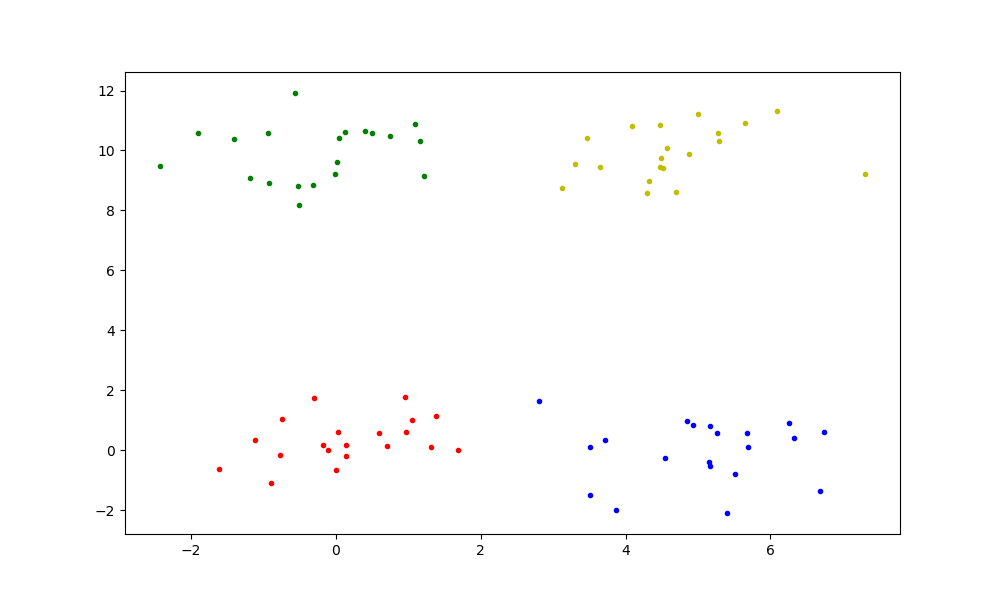
\includegraphics[width=\linewidth]{Images/classification.png}
  \caption{Classification}
\end{subfigure}%
\begin{subfigure}{.5\textwidth}
  \centering
  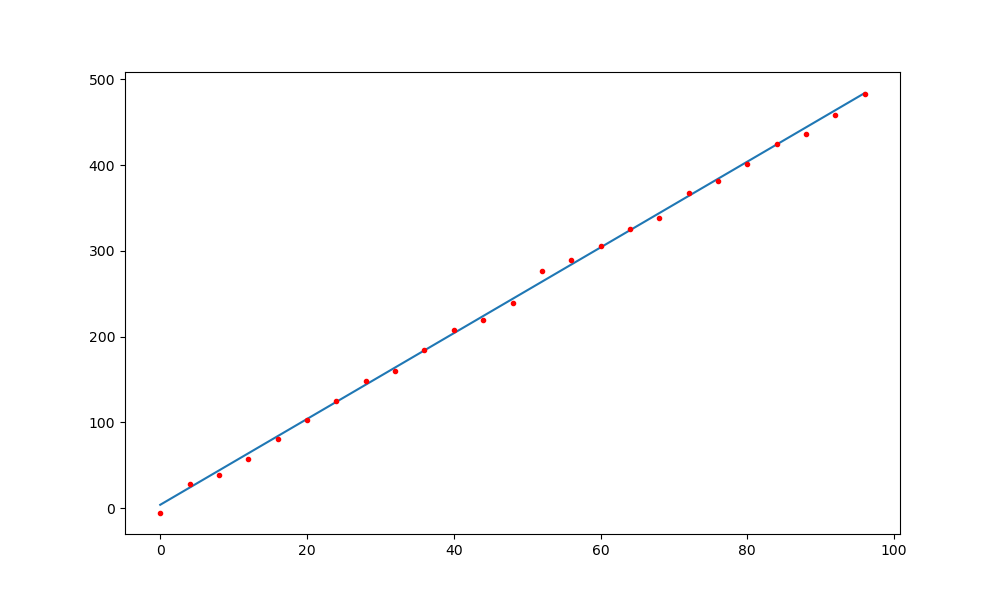
\includegraphics[width=\linewidth]{Images/regression.png}
  \caption{Regression}
\end{subfigure}
\caption{The two types of supervised learning}
\end{figure}

\subsection{Choosing a Model}

A machine learning model is evaluated on the basis of a loss function, which may be constructed differently for different problems. Naturally, we would want to select the model with the best accuracy or the least loss. There are two ways we can evaluate accuracy. We can check out how well the model predicts data we have already shown it, or training data. We can also show it brand new data or testing data. To test the model, often we split the data we have into training data and testing data by shuffling it and splitting. For this, we can use \code{sklearn.model\_selection.train\_test\_split}. We now train the model on the training data and evaluate it on the testing data. We evaluate many different models on their losses and accuracies. But how do we choose a split of the data we have? To do this, we can use cross validation. Cross validation is when we split the data into folds, and evaluate the model one by one keeping a fold for testing, while training on the rest. We then use the cumulative results to decide which model to pick. Crossvalidation can also be used to find the optimal hyperparameters for our model. More on the implementation of cross validation is available in the \href{https://scikit-learn.org/stable/modules/cross_validation.html}{scikit-learn docs}. However, cross validation means the model will have to be trained multiple times, so that might have to be a constraint to be considered.

\subsection{Generalization of an ML Model}

If our model simply memorizes the training data, we may not have good results as the outliers in the training data may induce weird biases to give awkward results during testing or when the model is deployed. So our model must learn sufficiently well from the data while still retaining a good ability to generalize to new data. If our model doesn't learn well enough from the training, it is said to underfit to the data. If our model does very well in training but poorly in testing, it is said to have overfit to the data. We need to find the right spot for the model to ensure a balance between training and testing accuracies. Epochs are a training pass through the training data, where the model attempts to learn or adjust its weights and parameters. In the plot below, we can see the fitting of the model during training increases with epochs. However the testing accuracy increases to a point and then starts dropping. The phenomenon to the left of the testing maximum is called underfitting and the right side of the maximum is overfitting. For a trained model in scikit-learn, we can calculate the training accuracy as \code{model.score(X\_train, y\_train)} and the testing accuracy as \code{model.score(X\_test, y\_test)}. There are more functions for complex metrics in scikit-learn. You can also use predictive analysis with probabilities for models which support them. 

\begin{figure}[H]
\centering
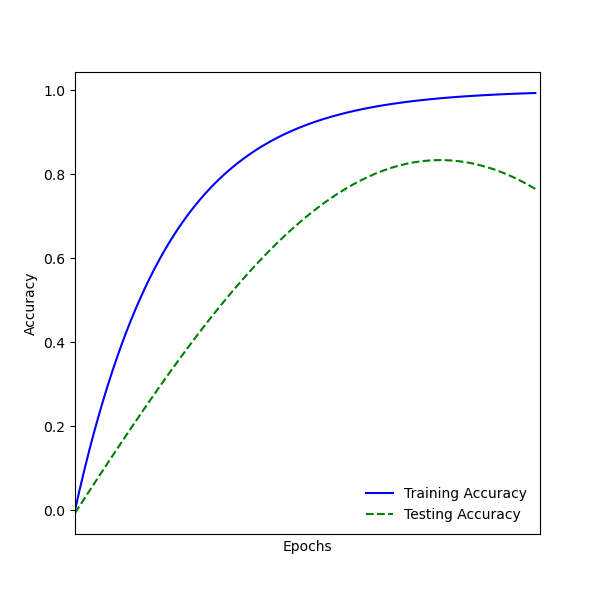
\includegraphics[width=.5\linewidth]{Images/curve_fit.png}
\caption{Training \& Testing Fit for a Model}
\end{figure}

This also introduces two important terms in machine learning - bias and variance. Bias is the inability of a machine learning model to fit to the true data, in other words, it is the training error. The difference in fits between different sets is called variance. Even though the training data and the testing data come from the same underlying distribution, often they don't have the same accuracy. In relation with the previous terminology, when the model has a high bias, it is said to be underfitting the data, and when the model has a high variance, it is said to overfitting the data. We have to optimize and find the ideal model which has the least possible variance for the minimum bias. 

\subsection{Confusion Matrix}

To analyse our model's successes and failures better, we make a confusion matrix. We can either use a normal binary two class confusion matrix, or even a multi class confusion matrix. With the example of the pre-existing datasets on the \code{sklearn} package, we load the iris and the breast cancer datasets. We train it with a supervised learning method - the polynomial support vector machine classifier and plot the correct classifications and the wrong classifications in a matrix. The true positives and true negatives (or correct classifications) are presented along the diagonal. Off diagonal results are the misclassfied erroneous vectors. If they are in the lower triangle of the matrix, it is a false positive, or a type I error. If they are in the upper triangle of the matrix, it is a false negative, or a type II error. Obviously, confusion matrices would be of size $n \times n$ for a $n$ classification problem.	

\begin{figure}[H]
\centering
\begin{subfigure}{.5\textwidth}
  \centering
  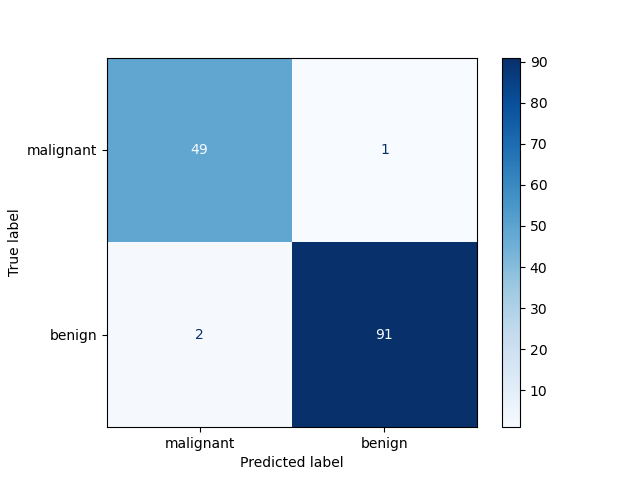
\includegraphics[width=\linewidth]{Images/twoclassconfmat.png}
  \caption{Binary Classification}
\end{subfigure}%
\begin{subfigure}{.5\textwidth}
  \centering
  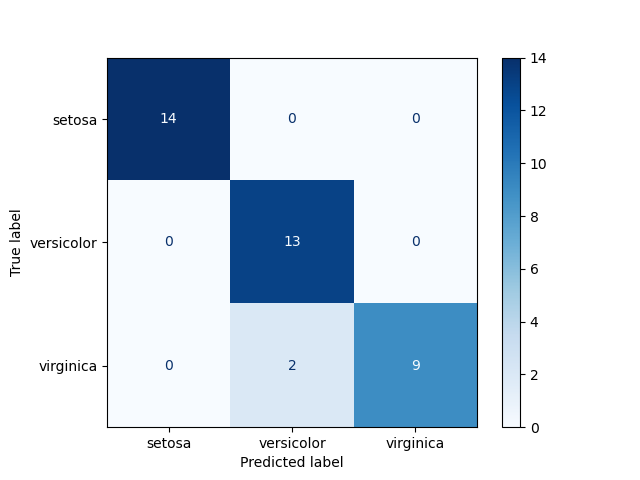
\includegraphics[width=\linewidth]{Images/threeclassconfmat.png}
  \caption{Multi Classification}
\end{subfigure}
\caption{Confusion matrices for the breast cancer and the iris dataset}
\end{figure}

\subsection{Fancier Metrics}

While the overall accuracy of the model can be calculated by summing the diagonal elements and dividing it by total elements, it often doesn't tell us the full picture. Heavily skewed data can affect our model. We can use the "sensitivity" or true positive rate or recall. It is the proportion of a class classified correctly. Similarly, we can define the "specificity" or the true negative rate. It is the proportion of wrong examples classified correctly, and would have more meaning for a binary classification problem. Precision is the ratio of correctly classified examples to all the examples classified so. As precision and recall are the most important metrics to draw from this, we use it to give one single number the F1 score, which is the harmonic mean of precision and recall.
$$F_1 \ score = \frac{2 \times precision \times recall}{precision + recall}$$
All of these metrics are summarized in one table here.

\begin{figure}[H]
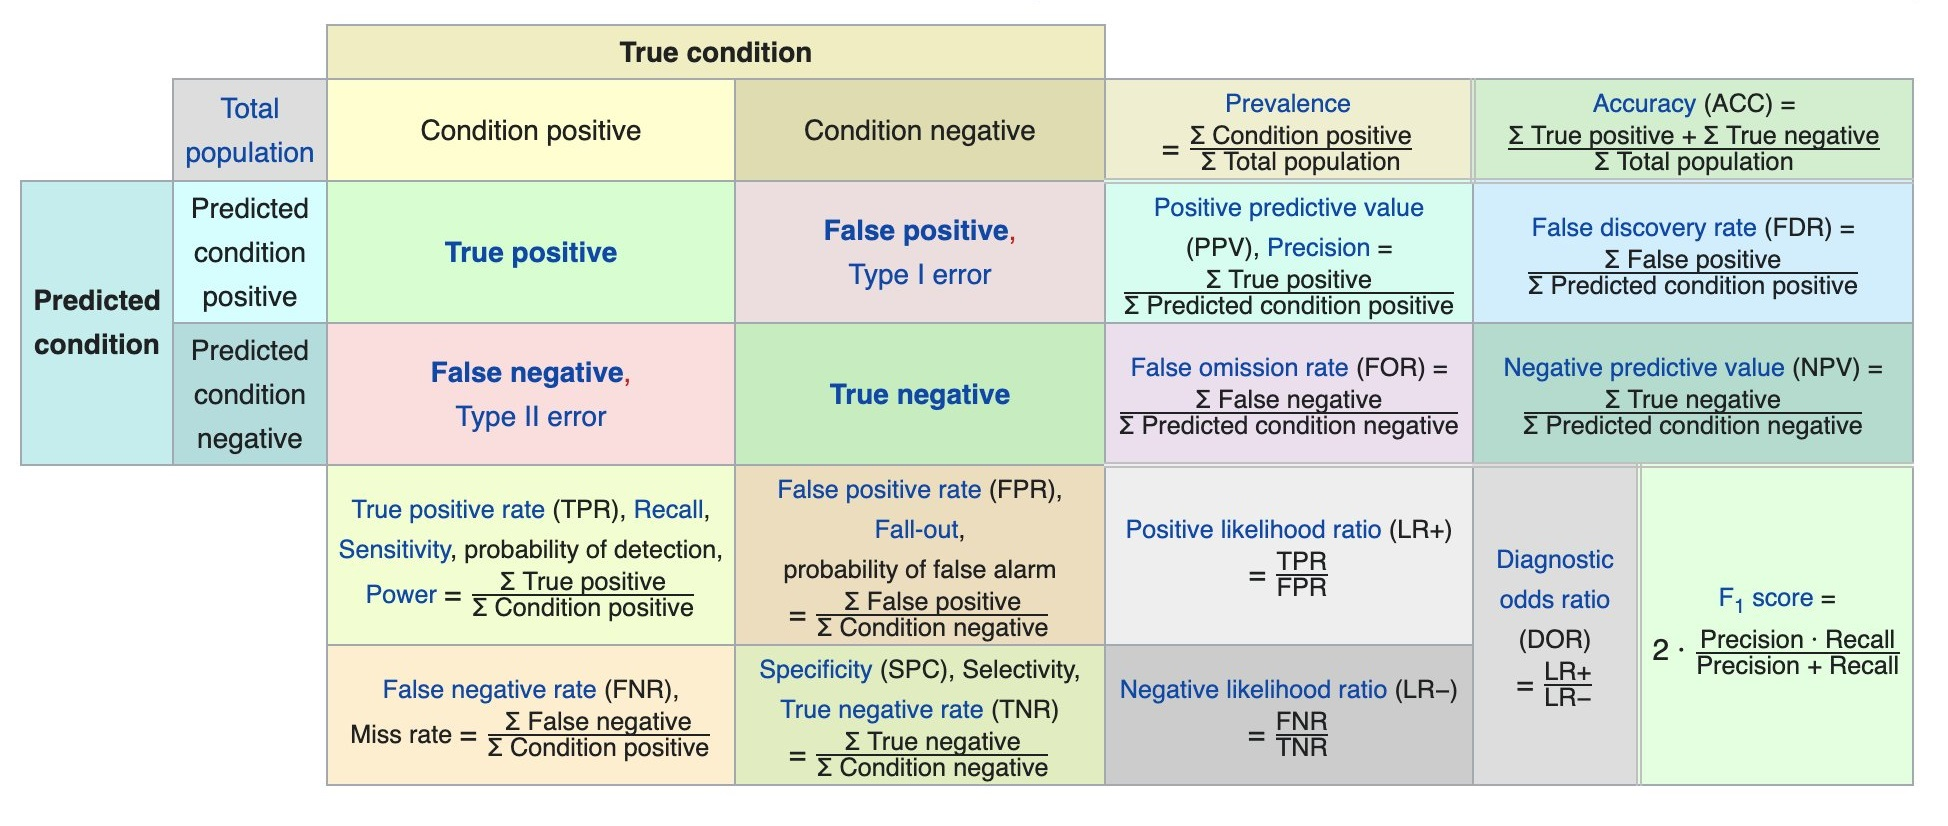
\includegraphics[width=\linewidth]{Images/confmatmetrics.jpeg}
\centering
\caption{The various metrics with which a Confusion Matrix can be analyzed}
\end{figure}

The \code{classification\_report} is a convenience function in scikit-learn to give all three metrics, the precision, the recall and the $F_1$ score in one function call.

\subsection{ROC Curves and AUC}

Often, our problem influences the parameters of a model. If we are forced to reduce the amount of false positives, or false negatives, then our model accommodates them by compensating elsewhere. Reducing false positives often increases false negatives and vice versa. We can also use this analysis to simply determine the best parameters for our model. This relationship is mapped by a plot between the true positive rate (\textit{sensitivity}) and false positive rate (\textit{1 $-$ specificity}). The plot is called receiver operator characteristic or ROC graph. For imbalanced data, it would be better to use precision instead of the false positive rate. For this, we construct a precision recall curve, as sensitivity can also be interpreted as recall. The area under the curve is another metric to help us deciding the best model to pick. The model with the largest area under the ROC curve does the best. A random classifier would have an AUC of exactly 0.5 for as it would get half the results right and half wrong. We can also use scikit-learn's \code{DummyClasssifier} which produces random predictions with the same proportions as classes in the training set.

\begin{figure}[H]
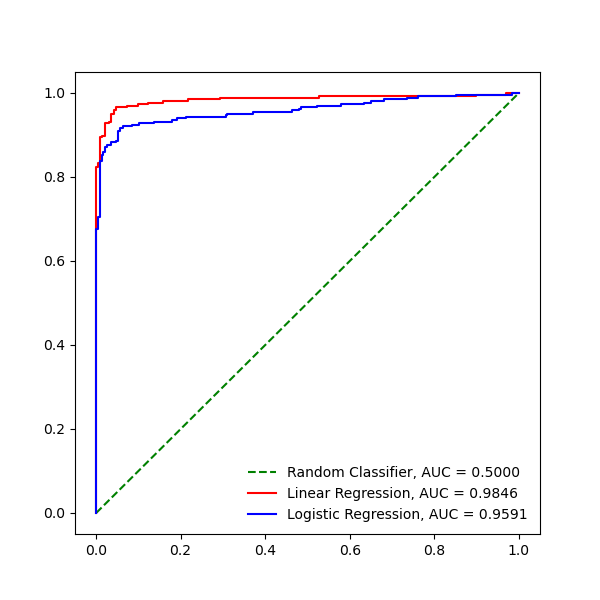
\includegraphics[width=0.7\linewidth]{Images/roc_curve.png}
\centering
\caption{ROC Curve for two linear models}
\end{figure}

\subsection{Hyperparameter Tuning}
Often, the model has some hyperparameters which control how well the model fits to the data or generalizes from it. Hyperparameters can be found manually in a rather tedious process or automated as well. \code{sklearn.model\_selection.GridSearchCV} takes in a python dictionary of possible hyperparamters and it will evaluate all combinations of these hyperparameters with cross validation. The attributes \code{best\_params\_} and \code{best\_estimator\_} will give us the parameters and the best model. Another option is to use the scikit-learn \code{RandomizedSearchCV} which randomly selects hyperparameters to search for. This method is not exhaustive unlike the Grid Search, and runs for a fixed number of iterations.


\section{Preprocessing and Dimensionality Reduction}

\subsection{Scaling}
Many machine learning models are sensitive to preprocessing of data. It is a common practice to scale the data for algorithms like MLP or SVM. Scikit-learn has implementations for various data scaling functions in the \code{sklearn.preprocessing} sub-package. The most common scaling methods in scikit-learn are \code{StandardScaler}, \code{MinMaxScaler}, \code{Normalizer} and \code{RobustScaler}. 

\begin{itemize}
\item[$\square$] Standard Scaler standardizes features by scaling it to a standard normal distribution. For every feature $x$ in the dataset, it does:
$$x' = \frac{x-\mu}{\sigma}$$
\item[$\square$] MinMax Scaler standardizes features by scaling them to a given range. This converts all the features in the data to between the range $[0, 1]$.
$$x'_i = \frac{x_i - x^{MIN}_i}{x^{MAX}_i - x^{MIN}_i}$$
\item[$\square$] Normalizer reduces the non-zero samples to a unit norm, which can either be $L_1$, $L_2$ or $\max$. It is used for clustering or for text classification.
\item[$\square$] Robust Scaler scales the data with the inter-quartile ranges about the median to ve robust to outliers in the data. To remove the outliers, on the other hand, you could go for clipping, changing the scale or \code{QuantileTransformer}.
\end{itemize}

\begin{figure}[H]
\centering
\begin{subfigure}{.5\textwidth}
  \centering
  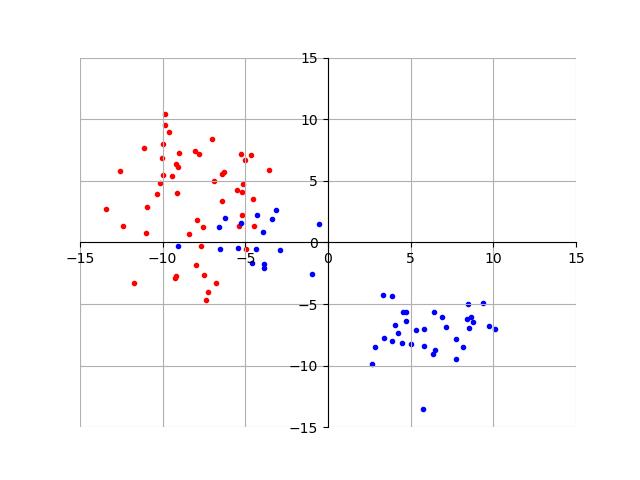
\includegraphics[width=\linewidth]{Images/orig_data_scaling.png}
  \caption{The original data}
\end{subfigure}%
\begin{subfigure}{.5\textwidth}
  \centering
  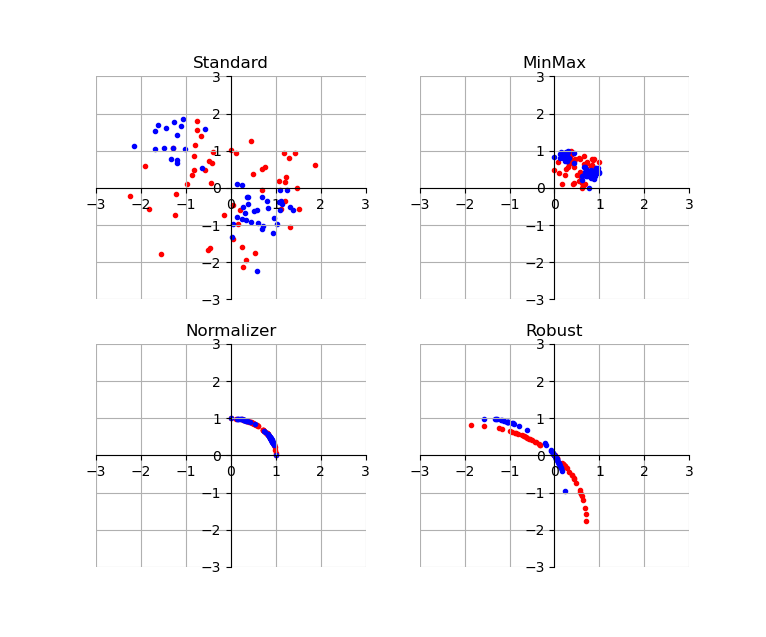
\includegraphics[width=\linewidth]{Images/scaled_data.png}
  \caption{Data after applying scale functions}
\end{subfigure}
\caption{Effect of scaling on data}
\end{figure}

The MinMax scaler was applied on an SVM with the radial basis function kernel, and a $C=100$. The model improved in performance on the train set after scaling the data, while managing to counter some variance.

\begin{figure}[H]
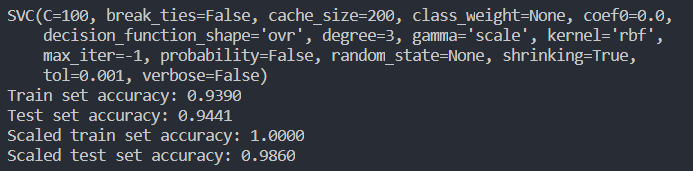
\includegraphics[width=0.8\linewidth]{Images/svm_with_scaling.png}
\centering
\caption{Effect of scaling on SVM}
\end{figure}

\subsection{Imputing}
Often missing values in data cause funky results as the model does not know what to do with it. Removing the vectors with missing inputs may work, but it can also cause a loss of data, especially when training data is really small. To remove data from a pandas DataFrame, \code{DataFrame.dropna()} is used. Another option is to consider removing the entire column, and this might be okay when most of the column is blank. This can be done with \code{DataFrame.drop()}. But the most common method of dealing with missing data is imputation. We replace the missing values with a representative guess of what it could be. This replacement can be 0, the median of the feature or the mean of the feature or any other suitable number. This can be done with \code{DataFrame.fillna()}, or with scikit-learn's \code{sklearn.impute.SimpleImputer}. The \code{KNNImputer} in the same submodule uses a more creative approach by comparing the nearest neighbors in the data with the other features, and uses this information to fill in missing values.

\subsection{Categorization and Discretization}
Often, some data is represented in the form of categories, as textual data, with strings or characters. This is often converted to a numerical format which the machine learning model can understand better. One way to do this is to club all the similar elements into a single number representing the class. This can be done with \code{sklearn.preprocessing.OrdinalEncoder}. For ordered data, this might be useful when represented properly, but in other categorical data, there are some categories more related to each other. To address this, we can use one-hot encoding, where every sample gets a vector which has an element 1 for the right category, and 0 everywhere else. In scikit-learn, this can be done with \code{OneHotEncoder}, and it returns a SciPy sparse matrix, not a NumPy array.

Discretization is when continuous data input is converted to a discrete value, usually for classification problems. One-hot encoded discretized features can make a model more expressive, while maintaining interpretability. For this the \code{sklearn.preprocessing.KBinsDiscretizer} can be used. Similarly, the \code{Binarizer} can be used with a threshold passed as a parameter to convert all the values to a boolean encoding.

Polynomial Features is a method with which a vector can be transformed to one in a higher feature space. While this is a preprocessing feature, it will be used in conjunction with many linear models to enable a richer set of functions to learn.

\subsection{Pipelines}
Scikit-learn also provides a pipeline to automate multiple data transformation procedures into a single step. All data transformation methods you wish to employ can be passed in the form of tuples to a pipeline which can be fit to the training data and transform it. It is mainly a convenience function. It allows for hyperparameter search for all estimators in the pipeline. Care must be taken to ensure there is no data leakage from the test set into the machine learning model. The pipeline must only transform the testing data and not fit to it.

\subsection{Principal Component Analysis}
\label{pca}
Principal component analysis or the Karhunen-Loeve transform is a dimensionality reduction technique used for feature extraction and data visualization. It is the orthogonal projection of data into a lower dimensional vector space known as the principal subspace. It can also be defined as the linear projection that minimizes average projection cost. 

Consider a dataset $\{x_n\}$ with $N$ elements, each of dimensionality $D$. Consider a unit vector $u_1$ belonging to this space, such that $u_1^T u_1=1$. Every data point is now projected onto a scalar as $u_1^T x_n$. Hence, the mean of the projected data would be $u_1^T \bar{x}$. The variance of the projected data is given by:
$$\frac{1}{N} \left( u_1^T x_n - u_1^T \bar{x} \right)^2 = u_1^T S u_1$$
And here, $S$ is the data covariance matrix, which is given by:
$$S = \frac{1}{N} \sum_{n=1}^N (x_n-\bar{x})(x_n-\bar{x})^T$$

Now the problem is a constrained maximization of $u_1^T S u_1$ with respect to $u_1$ with the condition $u_1^Tu_1=1$, and to this end, we will include a Lagrange multiplier, $\lambda_1$ and make the problem into maximizing this:
$$u_1^T S u_1 - \lambda_1 (1-u_1^Tu_1)$$

Setting the derivative to 0, we find that the quantity has a stationary point at:
$$Su_1=\lambda_1u_1$$
This suggests that $u_1$ is an eigenvector for the matrix S. Multiplying both sides by the transpose of $u_1$, we find that the variance is given by $\lambda_1$, and hence the variance will be maximum when we find the eigenvector corresponding to the largest eigenvalue of $S$. This eigenvector is the first principal component, and we can define additional principal components by choosing a different direction to maximise the variance in, and thus define the principal subspace as $\{ u_1, u_2, ..., u_m\}$. We can thus find the $m$ largest eigenvalues to find $m$ eigenvectors for the data. For a matrix of size $D \times D$ like the data covariance matrix, the algorithm is $\mathcal{O}(mD^2)$.

The iris dataset on scikit-learn is a four dimensional dataset, with the features \code{['sepal length', 'sepal width', 'petal length', 'petal width']}. To visualise this data, we use a seaborn pair plot. On the right side, we have the data along two of its principal components.

\begin{figure}[H]
\centering
\begin{subfigure}{.65\textwidth}
  \centering
  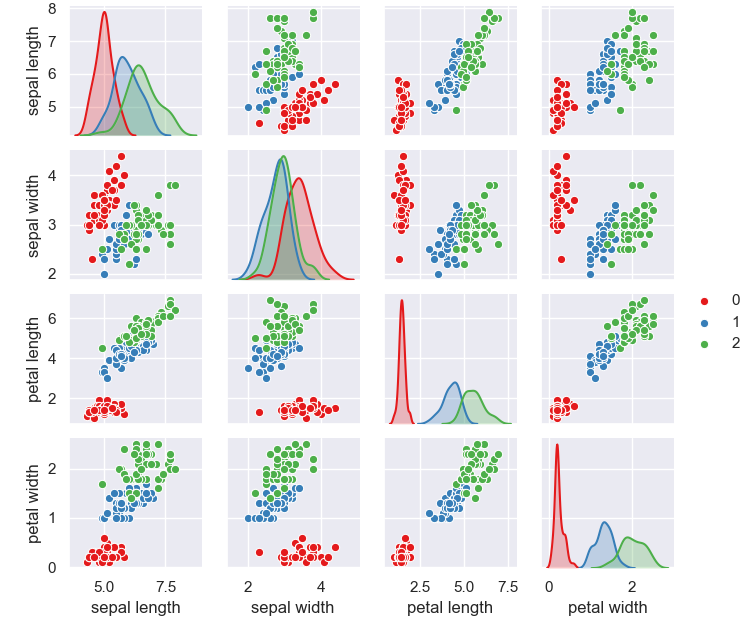
\includegraphics[width=\linewidth]{Images/iris_pairplot.png}
  \caption{Pair Plot}
\end{subfigure}%
\begin{subfigure}{.35\textwidth}
  \centering
  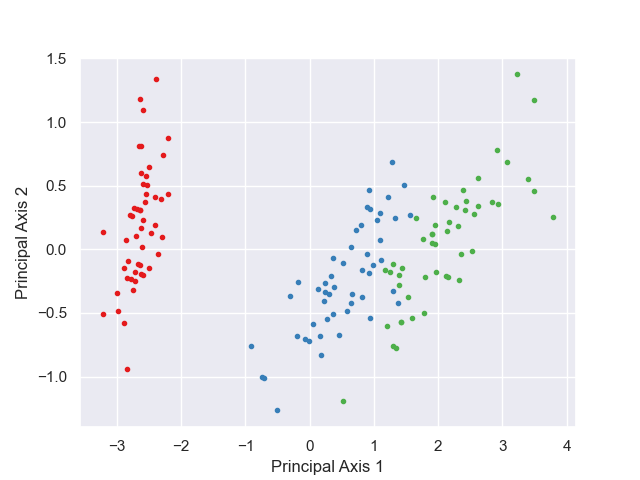
\includegraphics[width=\linewidth]{Images/principal_axes.png}
  \caption{Principal Components}
\end{subfigure}
\caption{PCA on the iris dataset}
\end{figure}

It's however, not easy to interpret the axes. They correspond to different directions in the data, and are often combinations of the original features. Here, we have the heatmap of the components, and their combination.

\begin{figure}[H]
\centering
\begin{subfigure}{.6\textwidth}
  \centering
  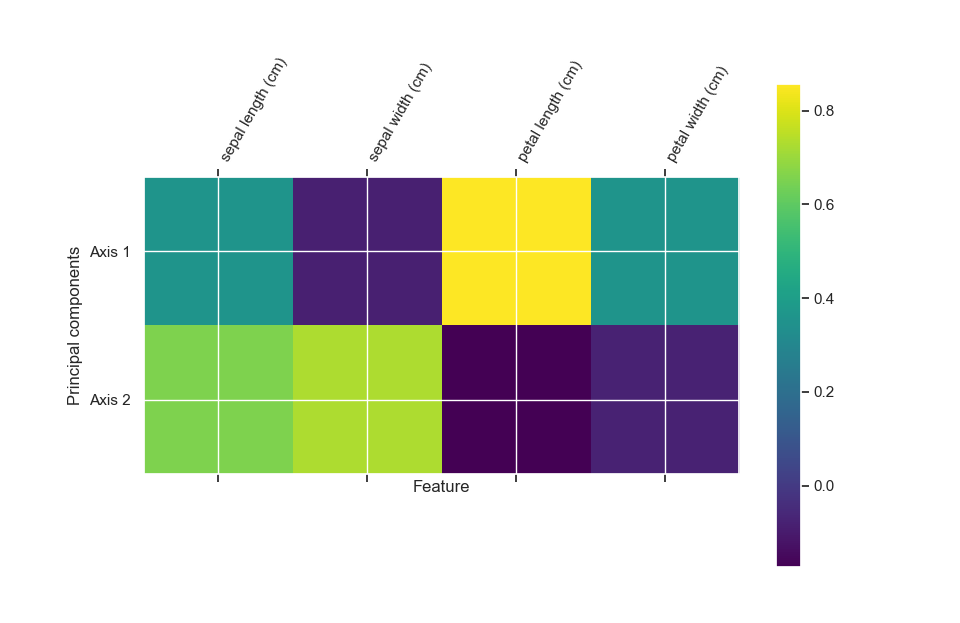
\includegraphics[width=\linewidth]{Images/iris_heatmap_pca.png}
  \caption{Heatmap of contribution}
\end{subfigure}%
\begin{subfigure}{.4\textwidth}
  \centering
  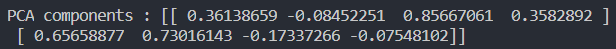
\includegraphics[width=\linewidth]{Images/iris_pca_components.png}
  \caption{Array of contribution}
\end{subfigure}
\caption{Contribution to principal components in the iris data}
\end{figure}

To choose the right number of component axes, we generally pick 2 or 3 to visualize the data. But this might not be the best way to go about things, so we set an explained variance threshold (usually around 95\%) and we use \code{numpy.cumsum()} to find the argument where we explain most of the variance, and consider those many dimensions.

More dimensionality reduction techniques will be seen in the unsupervised learning chapter.


\section{Supervised ML Algorithms}

\subsection{k-Nearest Neighbours}

It is the simplest machine learning algorithm. It works better for classification problems, rather than regression problems. Regression kNN algorithms still exist, but are used very rarely. It memorises the training set (yes). At test time, it iterates through the training set and finds the closest match to the vector presented to it. It classifies or regresses the new vector as belonging to the same class as the closest neighbour. This model has a hyperparameter $k$. Instead of immediately classifying the input vector as belonging to the nearest neighbour, the model now takes a vote between the $k$ nearest neighbours for the vector. The downside of this model is that it takes $\mathcal{O}(n)$ time during prediction, while $\mathcal{O}(1)$ time during training. Usually, this is the other way round with machine learning models, where prediction is supposed to be quick, but training can take its time. Nonetheless, it is still put to use in many character recognition or OCR tasks, where training data is quite small, and the test input is very similar to the training data.

Scikit-learn provides the class \code{sklearn.neighbors.KNeighborsClassifier}, which takes in an argument k for the kNN algorithm. We train this on the iris dataset from \code{sklearn.datasets.load\_iris}. We plot it for 6 values of k, namely, 1, 3, 7, 13, 21 and 51. Note how all values of k are odd - this is to reduce the possibility of a tie during the classification. Ties can be resolved by randomly picking a class. In the figures with low k, we see islands everywhere, and there are numerous overfitting artifacts as the model is very sensitive to outliers. Larger values of k smooth things out, but in an imbalanced dataset, the majority class might swamp the classification and affect performance. 

\begin{figure}[H]
\centering
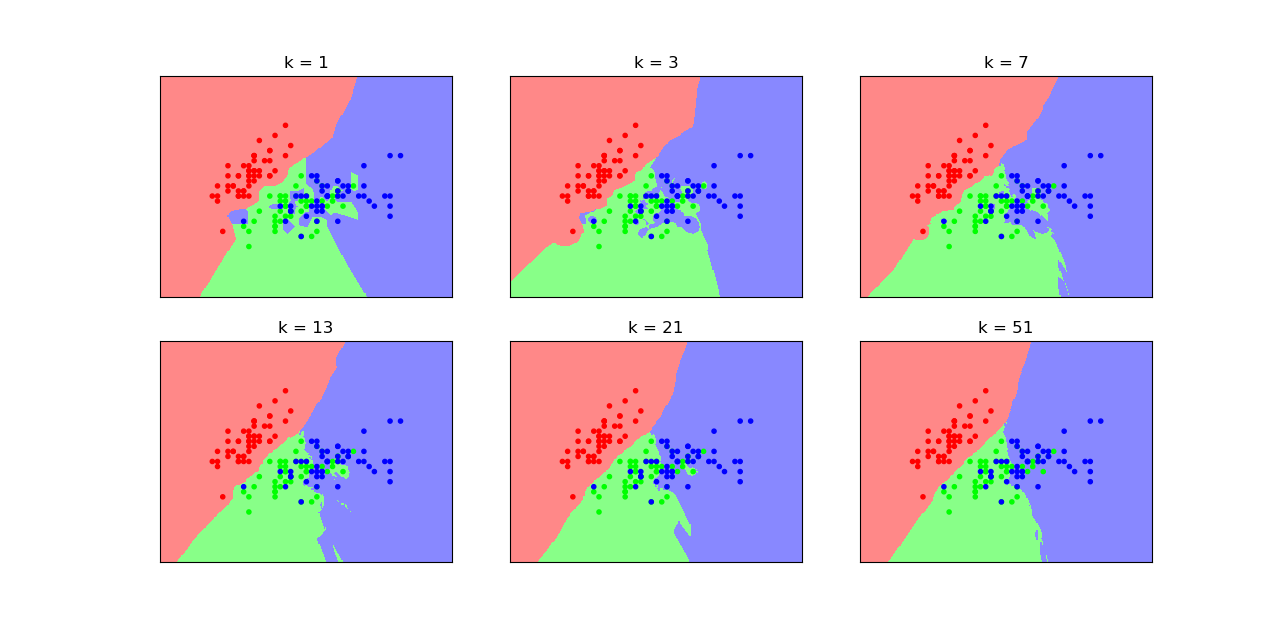
\includegraphics[width=\linewidth]{Images/knnclassifier.png}
\caption{kNN Classification}
\end{figure}

More mathematically, the kNN algorithm takes the input vector $v$, and makes a pass through the training data. For every vector $u_i$ in the training data, the norm of the difference is calculated as $l = ||u_i - v||$. The vectors $u_i$ for which $l$ is least is found out (by sorting or iterating or however), and the $k$ lowest $l$ values are pulled out separately. Among these $k$ values, a vote of the classification data, $y_1, y_2, ..., y_n$, is taken. The majority class in these k vectors is found and the input vector is classified as $\hat{y} = y_{max}$.

\clearpage
\subsection{Linear Models}

Linear models are used widely, as they are highly versatile, and can be used for regression and classification. A linear model learns a linear function to make a prediction. So if the model has $n$ parameters, the model predicts as below.
$$\hat{y} = w_1 x_1 + w_2 x_2 + ... + w_n x_n + b$$

\subsubsection{Linear Regression}
In linear regression, we try to find the line of best fit for the given data. For a set of $x$ and $y$ values, the seaborn library can quickly plot out the regression line with \code{sns.regplot(x, y)}. We also have to determine the goodness of fit for the regression line. To do so, we plot out the mean line of the $y$ data, $\bar{y}$ with x in the chart. 

\begin{figure}[H]
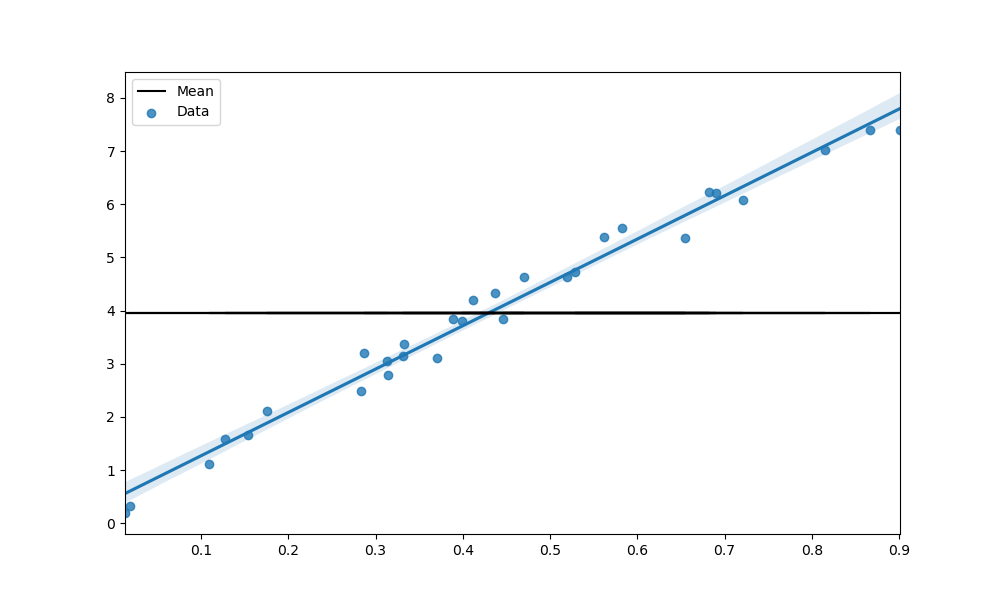
\includegraphics[width=0.7\linewidth]{Images/linear_reg.png}
\centering
\caption{Linear Regression}
\end{figure}

We now draw perpendiculars from the data we have to the mean line (i.e, find the residuals) and square their distances and sum them, in other words, we find this value.
$$l = \sum_{i=1}^n (\bar{y} - y_i)^2$$
The value $l$ that we found out is the sum of squared differences around the mean. Now we rotate the line to find an equation $\hat{y} = mx + c$. Now we find the new sum of squared \textit{residuals}, with $\hat{y}$ instead of $\bar{y}$ in the above equation. The line equation with the minimum sum of squared residuals is said to be the line of best fit or the regression line.

To evaluate the goodness of fit, we have a metric called $r^2$. To do this, we find the sum of squared differences around the mean, $l_{mean}$, and the sum of squared residuals around the line, $l_{line}$. 
$$r^2 = \frac{l_{mean} - l_{line}}{l_{mean}}$$
The $r^2$ score is a measure of how much of the data can be explained by the regression line. The larger the $r^2$ is, the better it explains the data. To explain if the $r^2$ is a good metric (\textit{sigh}), we use another metric the F score. The F score is the ratio between the variation in the dependent variable explained by the line to the variation in the dependent variable not explained by the line. To find this score, we use this equation.
$$F = \frac{(l_{mean}-l_{line})/(p_{line}-p_{mean})}{(l_{line})/(n-p_{line})}$$
Here, $n$ is the number of parameters in the data, $p_{line}$ is the number of parameters in the regression line and $p_{mean}$ is the number of parameters on the mean line. The various values of $F$ form the F distribution in statistics. The F distribution can be used to find a p-value for the amount of confidence we can have in our $r^2$ value. As all reliable p-values must be, the F score should be small.

In scikit-learn, we can use \code{sklearn.linear\_models.LinearRegression}. After training (fitting) a model, we can find the parameters of the model, or the equation of the line. The slope would be \code{model.coef\_} and the y intercept is \code{model.intercept\_}. These attributes can also be used for other linear models as well. The intercept is always a single float, but the coefficients are stored in a numpy array. The \code{model.score()} gives us the standard $r^2$ metric which we saw how to calculate above. The F score is also available in the \code{sklearn.feature\_selection.f\_regression}.

\subsubsection{Polynomial Features}
Polynomial features is a modification of regression where the existing features are mapped to a polynomial form. The problem is still a linear regression problem, but the input vector is now mapped to a higher dimensional vector which serves as a pseudo-input vector of sorts.
$$\textbf{x} = (x_0, x_1) \rightarrow \textbf{x'} = (x_0, x^2_0, x_1, x^2_1, x_0 x_1)$$
In this example, the input vector of 2 dimensions is mapped to a 5 dimensional input. The same ordinary least squares criterion which solves linear regression can be used, but the now instead of a line, we can fit polynomial functions to the data. In the graphic below, there is the nonchalant linear regression, with some higher degree 3 and degree 7 curves. The degree 15 curve is clearly sucking up to the data and overfitting as it jiggles across the graph. The original data was a randomly scattered $sin(x)$ plot.

\begin{figure}[H]
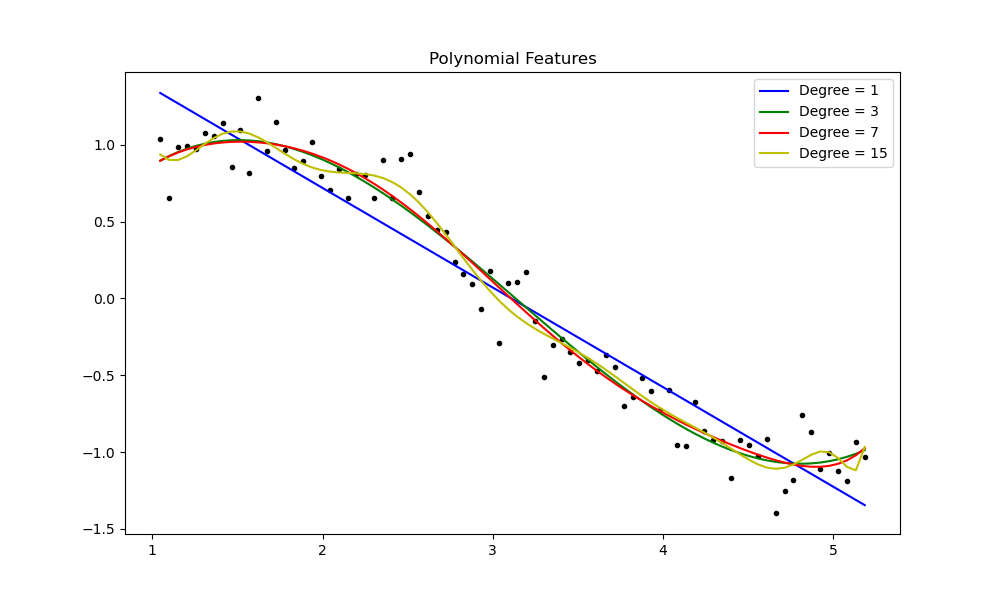
\includegraphics[width=\linewidth]{Images/poly_reg.png}
\centering
\caption{Polynomial Feeatures for the degrees 1, 3, 7, 15}
\end{figure}

\subsubsection{Ridge and Lasso Regression}
Ridge regression or Tikhonov regularization is a modified linear regression procedure. It adds a regularization term to the model to avoid overfitting. It reduces model complexity and forces the model to pick smaller parameters. This reduces the variance of the errors from the mean value. Here, it uses the $L_2$ regularization. Adding a regularization term reduces model complexity by increasing loss arbitrarily, hence forcing the model to pick a smaller set of parameters to minimize loss. The regularization parameter of ridge regression is $\alpha$ which when set to 0, is just plain vanilla linear regression. Increasing $\alpha$ slowly imposes the regularization term on the model, and values above 1 start forcing the model parameters towards zero. The ridge regression loss equation is as below.
$$l = \sum_{i=1}^n (y_i - \hat{y})^2 + \alpha \sum_{j=1}^p w_j ^2$$
The sum of squares of $w_i$ is added to the loss function with the hyperparameter $\alpha$ which pushes down its values. After the training, the prediction from the model is simply plugging in $X$ for the values of $W$ and $b$.

To prevent unfair scaling of the values in cases where $Y$ is very large compared to $X$ or vice versa, we normalize the values. When we push the values towards zero and towards each other, features of different scales will have different contributions to the $L_2$ penalty. Feature normalization is done by the following equation.
$$x'_i = \frac{x_i - x^{MIN}_i}{x^{MAX}_i - x^{MIN}_i}$$
This type of normalization is called MinMax scaling, and is different from the usual standard normalization. This makes all the input features to conform to the same scale between 0 and 1. Scikit-Learn has a class for this as well, in the \code{sklearn.preprocessing.MinMaxScaler} which we can \code{model.fit\_transform()}. The scaler must be fit to the training data, and should transform the test data. If the scaler is fit on the test data, it can cause data leakage and give results better than reality. 

Similarly, lasso regression also has the same regularization parameter, $\alpha$, only it uses $L_1$ regularization instead. The equation for lasso regression loss is given below.
$$l = \sum_{i=1}^n (y_i - \hat{y})^2 + \alpha \sum_{j=1}^p |w_j|$$
The parameter weights in $W$ are set to zero for least influential variables, and this results in a sparse solution. The lasso regression model works best when there is a lot of input data, but it seems as if only very few features actually contribute to the prediction. Ridge regression is better when a lot of the features contribute little by little to the overall prediction. If we just combine all the terms (because why not) to get a giant loss function, with ordinary mean squared error, lasso regularization and ridge regression, we get the hybrid Elastic-Net Regression. These regressions have different alphas for their purposes, and setting them to 0 can result in the corresponding regressions above.

Here, we compare ridge and lasso regression, with three values of $\alpha$, 0.01, 1 and 100, with vanilla regression as well. We plot out the coefficients in a graphic instead of the line to give more insight into what's happening inside. \code{sklearn.datasets.load\_boston} was used for the data to build the models.

\begin{figure}[H]
\centering
\begin{subfigure}{.5\textwidth}
  \centering
  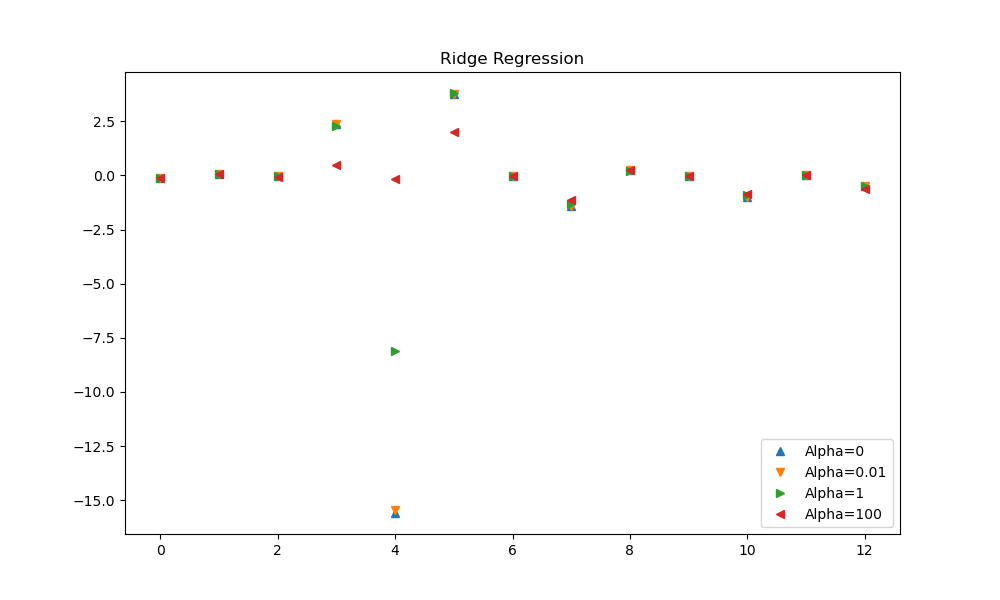
\includegraphics[width=\linewidth]{Images/ridge_reg.png}
  \caption{}
\end{subfigure}%
\begin{subfigure}{.5\textwidth}
  \centering
  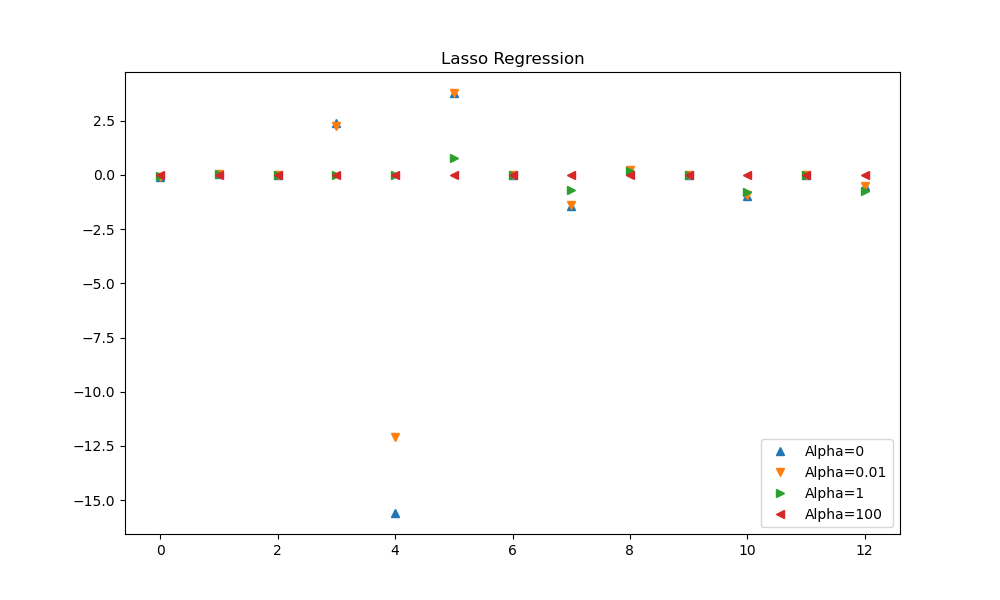
\includegraphics[width=\linewidth]{Images/lasso_reg.png}
  \caption{}
\end{subfigure}
\caption{Comparison of Ridge and Lasso Regression}
\end{figure}

With some careful analysis, you can find that all the useless parameters have been set to zero. The yellow and blue markers are close to each other for the most part, and they also tend to have the most extreme values. The green marker in an awkward middle position and the red marker hugs the zero line. The effect of regularization is seen in both types of regression with the coefficients being pushed to zero for large $\alpha$. Also check out scikit-learn's implementation of \href{https://scikit-learn.org/stable/auto_examples/linear_model/plot_lasso_coordinate_descent_path.html#sphx-glr-auto-examples-linear-model-plot-lasso-coordinate-descent-path-py}{coordinate descent}.

\subsubsection{Logistic Regression}
Unlike the other regression models, logistic regression is a classification algorithm. It is best suited to binary classification, which is done with a positive class and a negative class that is compared against a logistic curve fit to data. The logistic regression model still runs through the input features and finds an output vector, but runs the result through a non-linearity, the logistic curve. The logistic regression prediction is given by this equation.
$$\hat{y} = logistic(\hat{b} + \hat{w_1}x_1 + \hat{w_2}x_2 + ... + \hat{w_n}x_n)$$
$$\hat{y} = \frac{1}{1+exp(-(\hat{b} + \hat{w_1}x_1 + \hat{w_2}x_2 + ... + \hat{w_n}x_n))}$$
The logistic function transforms its real valued input vector to an output between 0 and 1, we can interpret the output as the probability that the feature belongs to the positive class. we can now add a threshold and use this for classification of the data. This is similar to the sigmoid activation function in neural networks. For better visualization, let us consider two features from the iris dataset, the sepal width and sepal length. Plotting them against each other, we fit this data on a logistic regression classifier and can see the decision boundaries. We can use all features, but this multidimensional data can't be visualized as easily.

\begin{figure}[H]
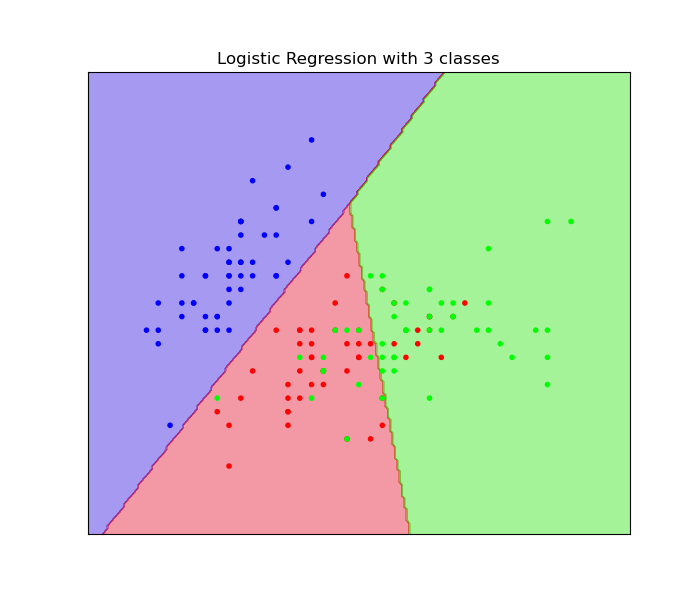
\includegraphics[width=0.7\linewidth]{Images/log_reg.png}
\centering
\caption{Logistic Regression with 2 features from 3 classes}
\end{figure}

Unlike linear regression, logistic regression doesn't use the concept of $r^2$ or residuals. Instead, it uses maximum likelihood estimation. A first probability curve given a set of features is made initially. The curve is used to calculate the likelihood of observing a positive class for every data point in the train set. The overall likelihood is now found by multiplying these likelihoods together. Now a new probability curve is found, and the process is repeated. The curve with the maximum likelihood is said to fit the data best, and is used for the classification. Let's try to formulate this mathematically. We first consider a logit function. $W$ is our weights row vector, and $X$ is the column vector of feature inputs. $b$ as we have seen before is the bias.
$$h(X) = W \cdot X + b$$
Now we interpret the logistic function output as a conditional probability. 
$$P(y=1|X; h(X)) = \frac{1}{1+e^{-h(X)}}$$
This can be re-written as follows.
$$WX = ln \left( \frac{P(y=1|X; h(X)}{1-P(y=1|X; h(X)} \right) $$
Being a binary classification problem we're considering here, it's either a positive class or a negative class, in other words success or failure, which brings us to the Bernoulli distribution. We have a single Bernoulli trial, and is a $n=1$ case in the binomial distribution. The number of successes is $k = {0, 1}$ for a single trial, which gives us this.
$$Y \sim B(1, p) = p^k (1-p)^{1-k}$$
Here $p$ is the threshold probability we use in the logistic curve based prediction. Therefore, likelihood, is given by this.
$$L(w|y) = \prod_{i=1}^n P(Y=y_i)$$
With product being a difficult method to use, we find the log-likelihood. This gives us our loss function to \textbf{maximize} unlike most other algorithms, and we use gradient ascent to this end.
$$loss = \frac{-1}{m} \sum_{i=1}^n y_i \
\log(h(X)) + (1-y_i) \log(1-h(X))$$
\code{LogisticRegression} in scikit-learn gives us a parameter C for controlling its regularization, which is set to $L_2$ by default. Higher C implies every individual point be classified correctly, while lower C means the model adjusts to clusters over points.

\subsection{Na{\"i}ve Bayes Classifier}
The na{\"i}ve Bayes classifier is a very simple classifier that uses Bayes theorem to determine probability of a vector belonging to a class. Consider data with $k$ classes and $n$ features. For an input vector $v$ of size $n$, we determine the probability of it belonging to a class $c_i$ by evaluating inverse probabilities with Bayes theorem. The probability hence is as follows.
$$P(c_i|v)  \propto P(c_i) P(v_1|c_i) P(v_2|c_i) ... P(v_n|c_i)$$
The $c_i$ having the largest probability is determined to be the class to which the vector $v$ belongs. 
$$\hat{y} = \arg \max_c P(c) \prod_{i=1}^n P(v_i|c)$$
This algorithm is very quick, and it allows the distribution of each feature to be analysed separately. While it is a decent classifier, it is a terrible estimator. The algorithm comes in three flavours in scikit-learn. These classes are all in the \code{sklearn.naive\_bayes}. \code{GaussianNB} can be applied to any continuous data, while \code{BernoulliNB} assumes binary data and \code{MultinomialNB} assumes count data (that is, that each feature represents an integer count of something, like how often a word appears in a sentence).

The gaussian algorithm assumes a gaussian likelihood of features. 
$$P(v_i|c_i) = \frac{1}{\sqrt{2 \pi \sigma^2_{c_i}}} exp \left( - \frac{(v_i - \mu_{c_i})^2}{2 \sigma^2_y} \right)$$

The multinomial algorithm works best in text classification, with multinomially distributed data. First a count of the number of times a feature $i$ appears in a class $c$ is taken. 
$$N_{yi} = \sum_{x \in T} x_i$$
Then the total count of all features for the class is taken.
$$N_y = \sum_{i=1}^n N_{yi}$$
Finally, the relative frequency count is taken with a smoothing parameter $\alpha$. It is called Laplace smoothing when $\alpha = 1$ and Lidstone smoothing when $\alpha < 1$.
$$\hat{\theta_{yi}} = \frac{N_{yi} + \alpha}{N_y + \alpha n}$$

The Bernoulli algorithm is a small variant of the multinomial version, but it uses this different decision rule to penalize the non-occurrence of a feature $k$ which is an indicator of a class $c$. 
$$P(v_k|c_i) = P(k|c_i) x_k + (1-P(k|c_i))(1 - x_k)$$

\subsection{Support Vector Machines}
Support vector machines are usually split into linear support vector classifiers (SVC) and kernelized support vector machines (SVM). It is highly effective in data with many features in large dimensions. They don't provide probability estimates directly, and is strictly a classification algorithm. As with almost every other classifier, we first take out the case of linear functions $f$, with the standard equation.
$$f(X) = W \cdot X + b$$
If the output of $f$ is a positive quantity, we classify the input vector as belonging to the positive class and vice versa for the negative class. To optimize this line, we have to position the decision boundary ideally.
Now we find the margin, the smallest distance between the decision boundary and the data points. We consider corresponding target values for the input vector $X$ as $t_n \in \{-1, 1\}$.  This allows $t_n f(X)$ to be positive for all data points in the training set. This margin can now be determined by finding the distance to the decision hyperplane from the data point, and that can be found by this.
$$d = \frac{t_n (W \cdot X + b)}{||W||}$$
The maximum margin solution for the SVM is now found by optimising $W$ and $b$ for solving this.
$$\arg \max_{w, b} \left\lbrace \frac{1}{||W||} \min_{n} [t_n (W \cdot X + b)] \right\rbrace$$
However we have made the assumption that the data is linearly separable, which is usually not the case. For this, we have a regularization parameter $C$ which controls how our not-so-clean data is classified. Larger values of $C$ means less regularization, which means the model tries to fit as many individual points as possible correctly, while smaller values is more tolerant of errors, and tries to maximize margins. In other words, for the linear SVC, we can formulate the problem as minimizing $l$.
$$l = \frac{1}{2} ||W||^2 + C \sum_{i=1} \max(0, t_n f(X))$$

Here, we can see the effect of C in the \code{LinearSVC} in scikit-learn which is a faster implementation of the support vector classifier for the special case of a linear kernel. It is based on the liblinear library, and scales as $\mathcal{O}(m \times n)$ where there are $m$ samples and $n$ features. 

\begin{figure}[H]
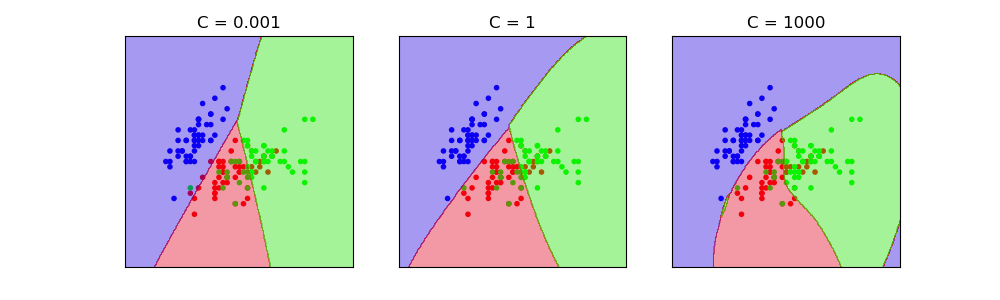
\includegraphics[width=\linewidth]{Images/linear_svm_C.png}
\centering
\caption{Effect of $C$ on Linear SVC}
\end{figure}

Another trick to make some non linearly separable data separable is to used kernelized SVMs. We can rescale our $W$ and $b$ to set the distance of the points closest to the margin as 1.
$$t_n (W \cdot X + b) = 1$$
Therefore all data points must satisfy this.
$$t_n (W \cdot X + b) \geq 1$$
For each of these $N$ points, we have constraints, which means we use Lagrange multipliers to optimize this loss. $\lambda$ will be the vector with the multipliers.
$$\mathcal{L}(W, b, \lambda) = \frac{1}{2} ||W||^2 - \sum_{n=1}^N \lambda_n \{ t_n (W \cdot X + b) - 1\}$$
Setting $\frac{\partial \mathcal{L}}{\partial W} = 0$ and $\frac{\partial \mathcal{L}}{\partial b} = 0$, we obtain two conditions.
$$W = \sum_{n=1}^N \lambda_n t_n X$$
$$0 = \sum_{n=1}^N \lambda_n t_n$$
Substituting these equations back, we get this maximization with respect to $\lambda$ problem.
$$\tilde{\mathcal{L}}(\lambda) = \sum_{n=1}^N \lambda_n - \frac{1}{2} \sum_{n=1}^N \sum_{m=1}^N \lambda_n \lambda_m t_n t_m K(x_n, x_m)$$
We have constraints, that all elements of our $\lambda$ vector are positive and dotting the $\lambda$ vector with $t_n$ should result in $0$. Also, in the equation, we have defined a kernel function $K$. This kernel function helps in making the SVM capable of learning high level features very similar to the polynomial features technique in linear regression. The linear kernel is the trivial case where $K(x_n, x_m) = x_n^T x_m$.

In the polynomial kernel, the kernel mapped is $\left\langle x, x' \right\rangle$ where $x'$ is the higher polynomial. In the scikit-learn implementation, we can use a parameter \code{degree} to control the dimension of the output space. Thus the kernel is $K(x_n, x_m) = (\gamma x_n^Tx_m + r)^d$, where $d$ is the degree, $r$ is a coefficient which we can control and $\gamma$ is the fit hyperparameter. Here a large $\gamma$ means complex, tightly constrained decision boundaries, while small $\gamma$ allows for a larger similarity radius. After transforming the space, it uses a linear classifier as we saw above to perform the classification. 

In the radial basis function kernel, the kernel is $K(x_n, x_m) = exp[-\gamma ||x_n-x_m||^2]$. The original input feature space is transformed into an exponentially decaying function of distance between the vectors. The $\gamma$ works the same way as the polynomial kernel.

To make predictions with a kernelized SVM, we have to modify the original linear equation into the modified feature space as well. The kernelized SVM has a training time complexity of between $\mathcal{O}(m^2n)$ and $\mathcal{O}(m^3n)$. Here, let's take a look at the various support vector machine kernels with various parameters on the first two features of the iris dataset.

\begin{figure}[H]
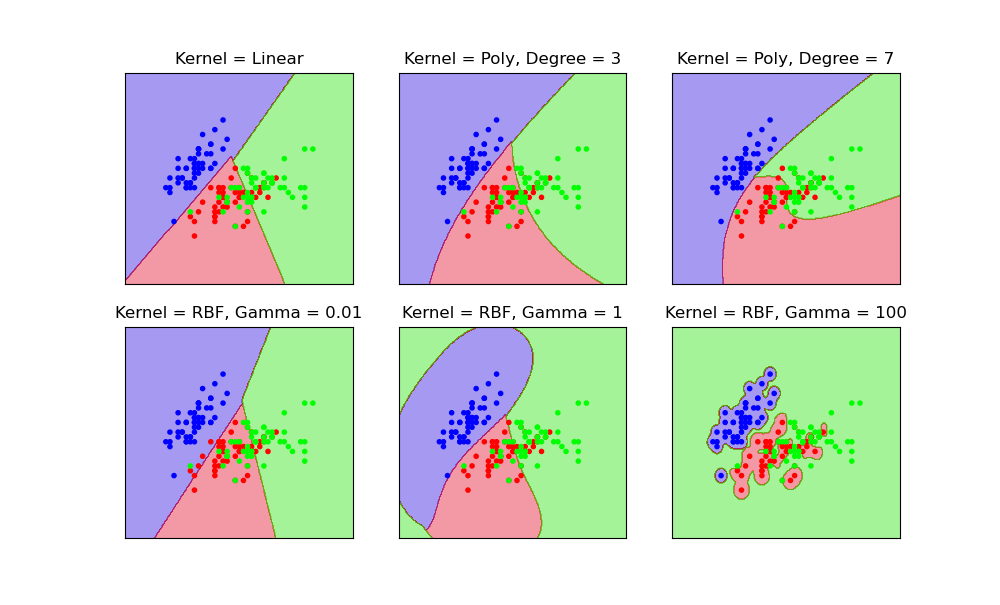
\includegraphics[width=\linewidth]{Images/kernel_svm.png}
\centering
\caption{SVM with different kernels}
\end{figure}

Normalization of data can have a huge impact on SVM performance, so be sure to apply \code{MinMaxScaler()} to the data before using SVMs. While SVMs work really well for multidimensional data, their efficiency decreases as training set increases.

\subsection{Decision Trees}

Decision trees are powerful models which learn a series of hierarchical questions which lead to a decision. The node at the top of the tree is called root node, and the final nodes at the bottom are called leaves. The intermediate nodes and decision making is done based on the features in the training set. They are very easy to interpret and often require very little data cleaning. It can handle both numeric and categoric data. However decision trees tend to overfit and may create biased trees in unbalanced datasets. The complexity of a decision tree construction is $\mathcal{O}(n_{features} n_{samples} \log(n_{samples}))$. The trees constructed need not necessarily be balanced, as they conduct a greedy search for the feature that offers the largest reduction in entropy. The query time is still $\mathcal{O}(\log(n_{samples}))$. 

A decision tree is constructed with three measures of impurity - entropy, misclassification or Gini index. At each decision node, we calculate the probability of the positive class and the negative class. Entropy being a measure of information, will tell us if each split is useful or not. Let's consider $N$ classes for our data. The entropy is defined as based on the proportions of elements of each class, represented by $p_1, p_2, ..., p_N$.
The entropy is given by:
$$H(X) = - \sum_{i=1}^n p_i \log_2 (p_i)$$
The Gini index is given by:
$$H(X) = \sum_{i=1}^n p_i (1-p_i)$$
And the misclassification coefficient is given by:
$$H(X) = 1 - \max(p_i)$$

At each decision node $m$, let's say we have $A$ as our data set for that node. The individual training vectors and label vectors are still represented by $X$ and $y$. We have the split as $\theta = (i, t)$ with $i$ the feature being considered for the split and $t$ the split threshold. We split the data as:
$$A_{left} = (X, y) \ |\  x_i <= t$$
$$A_{right} = A - A_{left}$$
Now we calculate the node impurity with the impurity functions defined above.
$$G(A, \theta) = p_{i, left}H(A_{left}) + p_{i, right}H(A_{right})$$
If pick the parameters which minimise impurity.
$$\theta *  = \arg \min _{\theta} G(A, \theta)$$
Continue this recursively until the maximum depth is reached, or the new split doesn't look better than the previous one.

Classification is just a simple stride down the tree, which can be interpreted very easily. We can even visualize the tree on scikit-learn with \code{sklearn.tree.plot\_tree(model)}. To train the model, we can again use the same module but we call the classifer, \code{sklearn.tree.DecisionTreeClassifier()}. 

\begin{figure}[H]
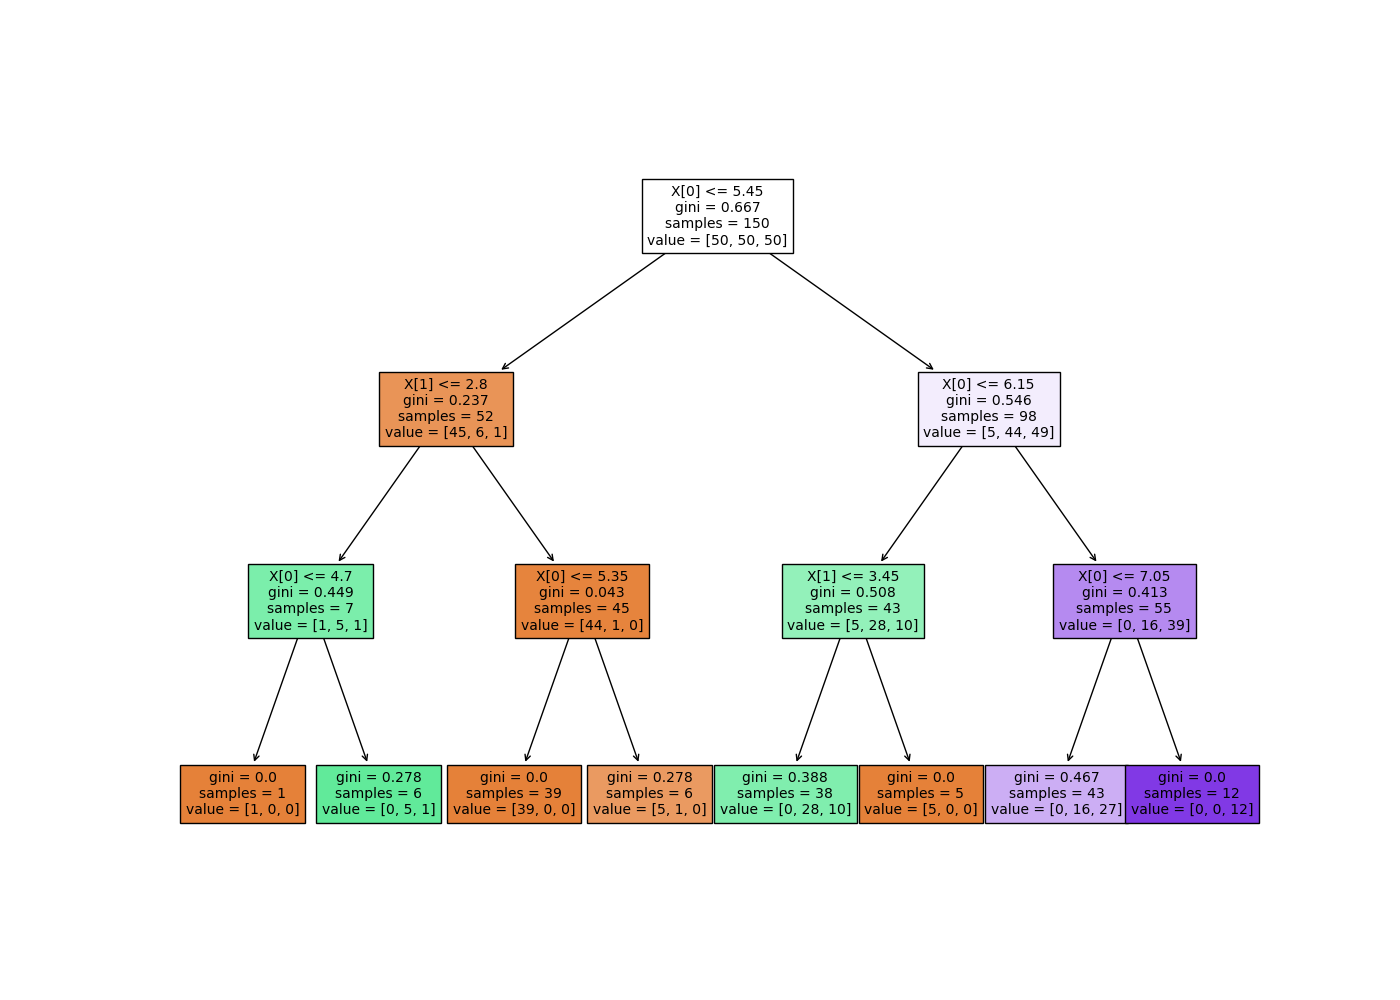
\includegraphics[width=\linewidth]{Images/tree_small.png}
\centering
\caption{Depth 3 Decision Tree on the iris dataset}
\end{figure}

Decision trees can also be used for regression problems. For regression problems with a decision tree in scikit-learn, use \code{sklearn.tree.DecisionTreeRegressor()}. At a node $m$ with $N_m$ observations, we can use the mean squared error or $L_2$ loss to minimize mean and to determine splits. $X$ is the training data at the node in question. 
$$\bar{y}_m = \frac{1}{N_m} \sum_{i \in N_m} y_i$$
$$H(X) = \frac{1}{N_m} \sum_{i \in N_m} (y_i - \bar{y}_m)^2$$
We can also use the mean absolute error or $L_1$ loss, but now we use the median instead of the mean.
$$\tilde{y}_m =  \underset{i \in N_m}{median} (y_i)$$
$$H(X) = \frac{1}{N_m} \sum_{i \in N_m} |y_i - \bar{y}_m|$$

One drawback of decision trees is that they love to overfit to the training data. Some dimensionality reduction technique would help combat this. Converting sparse data to a better format would also improve training time. Another common technique is to limit the depth of the tree. This is called pre-pruning. Here, we can look at the tree overfitting heavily in the default settings. The plot of the default tree is \href{https://github.com/sbalan7/ML-and-Stats/blob/master/Images/tree_hi_res.png}{here}. The decision surfaces for decision trees look rectangular because of the sharp thresholds in the decision nodes.

\begin{figure}[H]
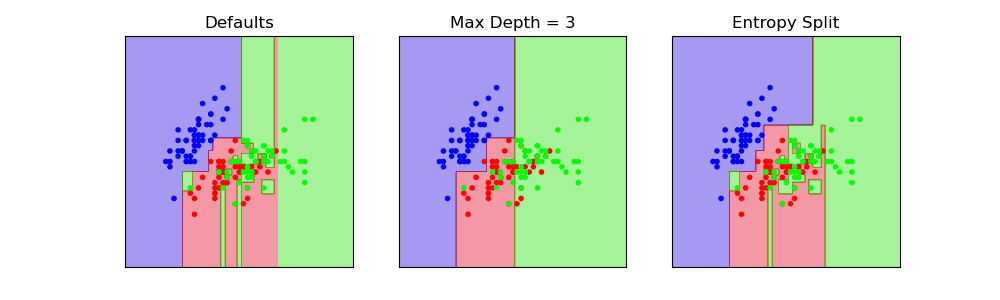
\includegraphics[width=\linewidth]{Images/decision_tree_surfaces.png}
\centering
\caption{Decision Surfaces for Decision Trees}
\end{figure}

Minimal cost-complexity pruning is another algorithm used to cut out leaves in the tree to prevent overfitting. For every possible decision tree with pruned leaves, we evaluate the cost complexity measure. Here, $T$ is the tree, $n_L$ is the number of leaves in the tree and $J(T)$ is an method to calculate misclassification, in simpler terms a loss function. $\alpha$ is a tunable hyper parameter, which must be found through cross validation.
$$J_{\alpha}(T) = J(T) + \alpha n_L$$

To find the optimal $\alpha$, first we start with a tree built on all the data, and start with $\alpha=0$. Now we increase $\alpha$ till pruning the leaves gives us a lower $J_{\alpha}$. We now test the different trees with cross validation at their optimal $\alpha$s and find which tree does well consistently across the cross validation.

\subsubsection{Random Forests}
Random Forests are another method to counter overfitting in decision trees. We build multiple trees, and use their collective decision to decide the classes. First, we make a bootstrapped dataset, by bootstrap aggregation or bagging. First, we draw a bootstrap sample $Z*$ of size $N$ from the training data $Z=(X, y)$. Now we grow a decision tree $T_i$ with $Z*$. We repeat this process $n$ times if we want to populate our forest with $n$ trees. If we wanted to make a classification, then we take the majority vote across all the $n$ trees in the forest. If we want to make a regression prediction, we do so by:
$$\hat{y} = \frac{1}{n} \sum_{i=1}^n T_i(X)$$
In scikit-learn, the random forest implementation is \code{sklearn.ensemble.RandomForestClassifier()}. Scikit-learn also has a regressor in \code{sklearn.ensemble.RandomForestRegressor()} or a collection of totally random trees in \code{sklearn.ensemble.RandomTreesEmbedding()}.

\subsubsection{Bagging Classifier}
Bagging algorithms build several instances of a black-box estimator on random subsets of the original training set. They help in introducing randomization to the training procedure, which almost always helps in model generalization. Bagging methods work better with large strong models such as deep decision trees, as opposed to boosting, which helps weaker models like short decision trees.

\subsubsection{AdaBoost}
AdaBoost is one of the boosted tree learning approaches which also combines the learning from many weak learners to produce an accurate result. AdaBoost uses stumps, which are decision trees, but with only one decision node, which is also the root node. AdaBoost, which is short of Adaptive Boosting, does the adaptation with a sample sample weight column to the data. This will tell us which stumps did a better job, and all also help us make better classification stumps. Initially we set the weighting of each sample equally, as $1/N$ where we have $N$ samples in the data. 
$$w_i = 1/N$$
Now we use the Gini impurity, or entropy to calculate the best split of data. Let's say this classifier stump we trained is $T(x)$. We find the total error in the best split. It can be found by summing up the weights of all the incorrectly classified samples and normalizing it. 
$$e = \frac{\sum_{i=1}^N w_i I(y_i \neq T(x_i)))}{\sum_{i=1}^N w_i }$$
This will be $0$ for a perfect stump, and $1$ for the worst stump. The total error is also used to weight stumps which are better at classification with a higher say in the final vote. The amount of say a stump has is given by this measure, where $e$ is the total error:
$$a = \frac{1}{2} \log{\frac{1-e}{e}}$$
Finally, we update the weights of the samples, by increasing weights for the incorrectly classified samples. Sometimes, the other weights are reduced to maintain a constant weight for the sum total of weights, but that is unnecessary if it will be normalized. 
$$w_i' = w_i \exp{(a I(y_i \neq T(x_i))}\ \forall \ i \in (X, y)$$
We now repeat this process for as many stumps as we want to have in our forest.

AdaBoost is a meta-learning algorithm, because it uses information about incorrectly classified samples to build better copies of the classifier. In scikit-learn, AdaBoost is implemented for classification problems with \code{sklearn.ensemble.AdaBoostClassifier()} and \code{sklearn.ensemble.AdaBoostRegressor()} for regression problems.

\subsubsection{Gradient Boosting}
Gradient Boosting is similar to AdaBoost, but we construct trees of fixed sizes instead of stumps. With the example of a binary classification problem, first we calculate the log-odds of a class. We now convert this to a probability with a logistic function.
$$p_+ = \frac{e^{\log{(+/-)}}}{1 + e^{\log{(+/-)}}}$$
This gives us the predicted probability for the positive class. Now we calculate the residuals with this probability for every sample in the dataset. Now we build a decision tree of fixed size, by limiting the total number of leaves in the tree. Each leaf will have a set of the residuals from the dataset. To make a transformation of these into probabilities, we first calculate leaf output value with this formula:
$$o = \frac{\sum r_i}{\sum p_i(1-p_i)}$$
$p_i$ is the previous probability for every sample in the leaf which is initially just the log-odds we initialised the model with. $r_i$ is the residual for every sample in the leaf. Finally, we calculate the probability by:
$$p = logistic(p_+ + lr \times o(x_i))$$
We use a learning rate to control our algorithm and prevent it from overfitting. We repeat the above process by calculating new residuals, then growing a new tree, and continue till we reach a user defined limit or no progress is being made.

Gradient Boosting is implemented in scikit-learn as \code{sklearn.ensemble.GradientBoostingClassifier()} for classification and \code{sklearn.ensemble.GradientBoostingRegressor} for regression.

Here there is a decision boundary plot of random forests, AdaBoost and gradient boosting trained on two features of the iris dataset.

\begin{figure}[H]
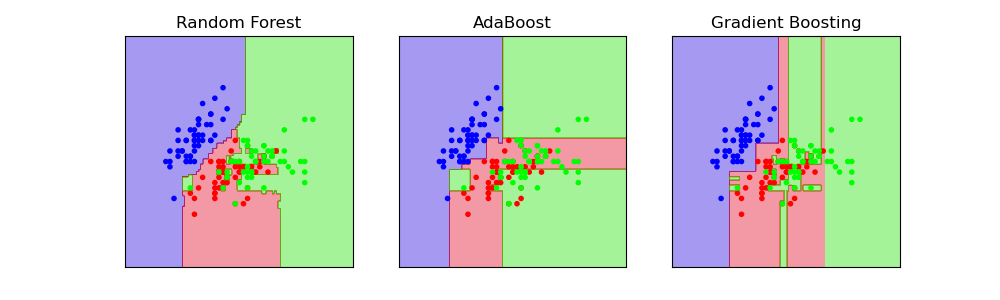
\includegraphics[width=\linewidth]{Images/random_boosting_trees.png}
\centering
\caption{Comparison of Random and Boosted Decision Trees}
\end{figure}

\subsection{Neural Networks}
We have one of the most powerful techniques for learning, and in scikit-learn, \code{sklearn.neural\_network} has a set of functions for this. Scikit-learn supports multi-layer perceptron feed forward networks. But this whole concept deserves its own separate set of notes, so do go check those out \href{https://sbalan7.github.io/assets/notes/deeplearning.pdf}{here}. While artificial neural networks as shown here aren't better than other algorithms here as such, their modifications are extremely powerful and put a large variety of applications.

\subsection{Summary}

\begin{itemize}
\item[$\square$] \textbf{Nearest neighbors} are good for small datasets, good as a baseline, easy to explain.
\item[$\square$] \textbf{Linear models} are a go-to as a first algorithm to try, good for very large datasets, good for very high dimensional data.
\item[$\square$] \textbf{Na{\"i}ve Bayes} are meant only for classification. It is faster than linear models, good for very large datasets and high-dimensional data. Often less accurate than linear models.
\item[$\square$] \textbf{Support vector machines} are more powerful for medium-sized datasets of features with similar meaning. Require scaling of data, sensitive to parameters.
\item[$\square$] \textbf{Decision trees} are very fast, don't need scaling of the data, can be visualized and easily explained.
\item[$\square$] \textbf{Random forests} almost always perform better than a single decision tree, very robust and powerful. Don't need scaling of data. Not good for very high-dimensional sparse data.
\item[$\square$] \textbf{Gradient boosted decision trees} are often slightly more accurate than random forests. Slower to train but faster to predict than random forests, and smaller in memory. Need more parameter tuning than random forests.
\item[$\square$] \textbf{Neural networks} can build very complex models, particularly for large datasets. Sensitive to scaling of the data and to the choice of parameters. Large models need a long time to train.
\end{itemize}

Here's a comparison of time taken by some different classification models in scikit-learn, in a linear scale and a log scale. The breast cancer dataset from scikit-learn was used. For plots of the wine dataset or the iris dataset, check out this \href{https://github.com/sbalan7/ML-and-Stats/tree/master/Images/Sup_Learn_Classifiers}{link}. All the * marked algorithms use their default scikit-learn settings. The algorithms used are k-Nearest Neighbours ($k=5$), Logistic Regression, Gaussian Na{\"i}ve Bayes, SVM with RBF kernel, SVM with degree 5 polynomial features, Decision Tree, Random Forest, AdaBoost and Gradient Boosting.

\begin{figure}[H]
\centering
\begin{subfigure}{.5\textwidth}
  \centering
  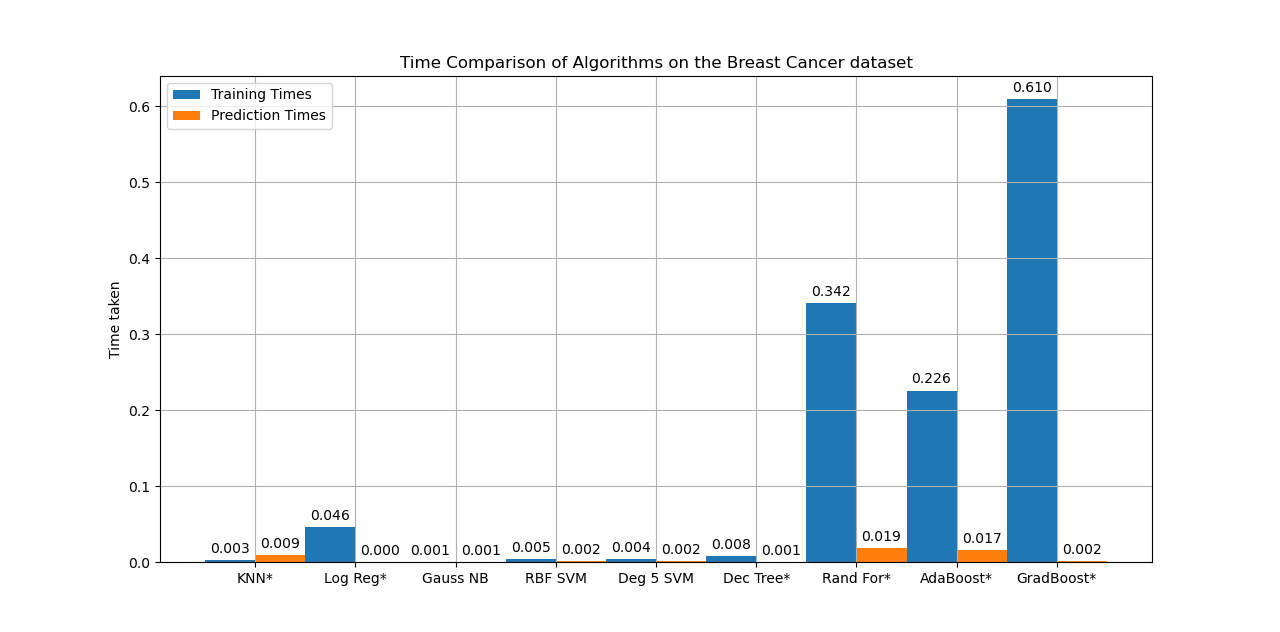
\includegraphics[width=\linewidth]{Images/sup_learn_comp_lin.png}
  \caption{Linear Y axis}
\end{subfigure}%
\begin{subfigure}{.5\textwidth}
  \centering
  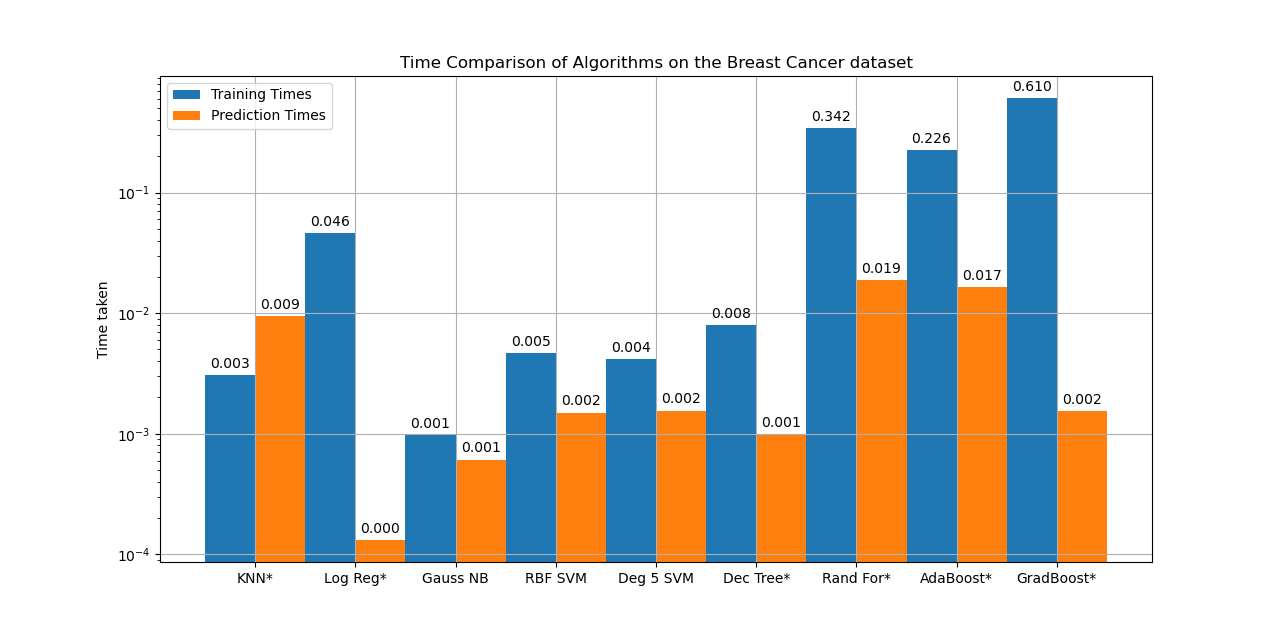
\includegraphics[width=\linewidth]{Images/sup_learn_comp_log.png}
  \caption{Logarithmic Y axis}
\end{subfigure}
\caption{Comparison of Supervised Learning Classifiers}
\end{figure}

And the score comparison for the same dataset:

\begin{figure}[H]
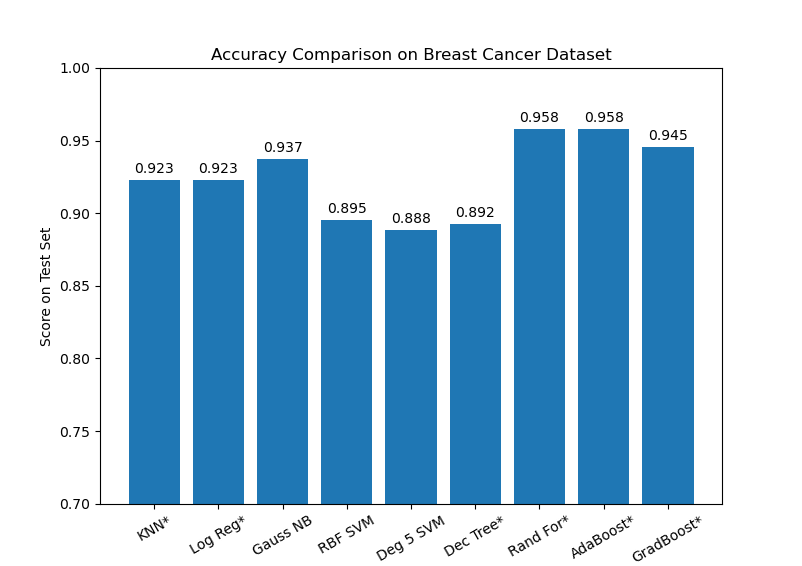
\includegraphics[width=0.5\linewidth]{Images/sup_learn_comp_sco.png}
\centering
\caption{Score comparison for Supervised Learning Classifiers}
\end{figure}

And decision boundaries for some other algorithms with different data and their test accuracies inset.

\begin{figure}[H]
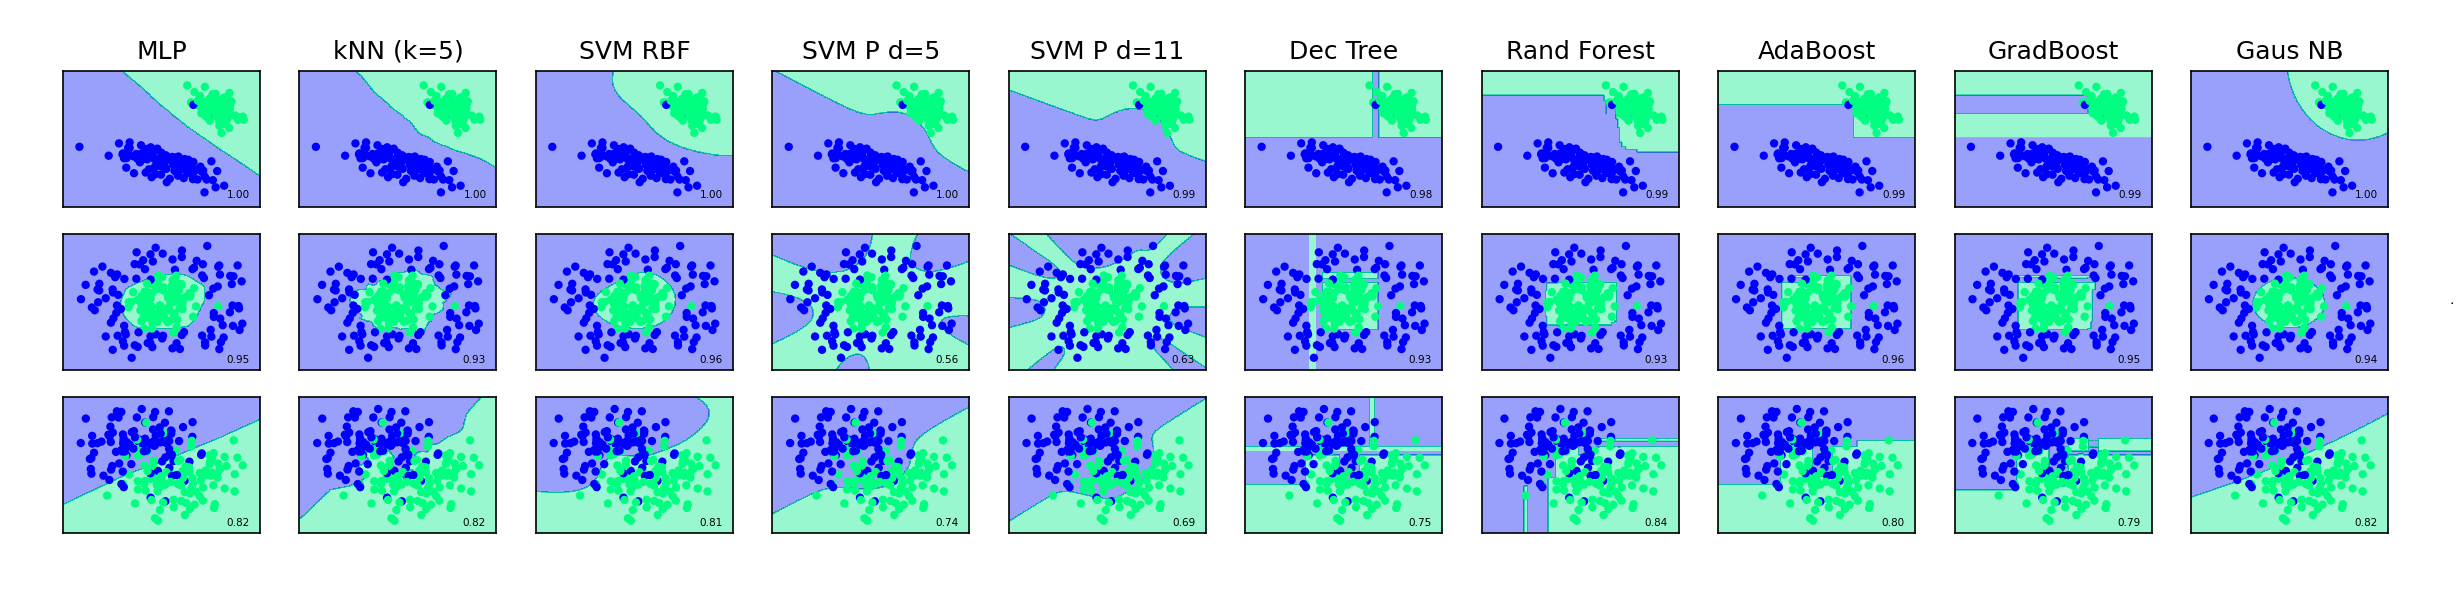
\includegraphics[width=\linewidth]{Images/sup_learn_decisions.png}
\centering
\caption{Supervised Learning Algorithms' Decision Boundaries}
\end{figure}

Similarly, here's a comparison for regression. The Boston housing Prices dataset was used. Again, all the * marked algorithms use their default scikit-learn settings. The algorithms used here are Linear Regression, Ridge Regression, Lasso Regression, SVM with RBF kernel, SVM with degree 5 polynomial features, Decision Tree, Random Forest, AdaBoost and Gradient Boosting.

\begin{figure}[H]
\centering
\begin{subfigure}{.5\textwidth}
  \centering
  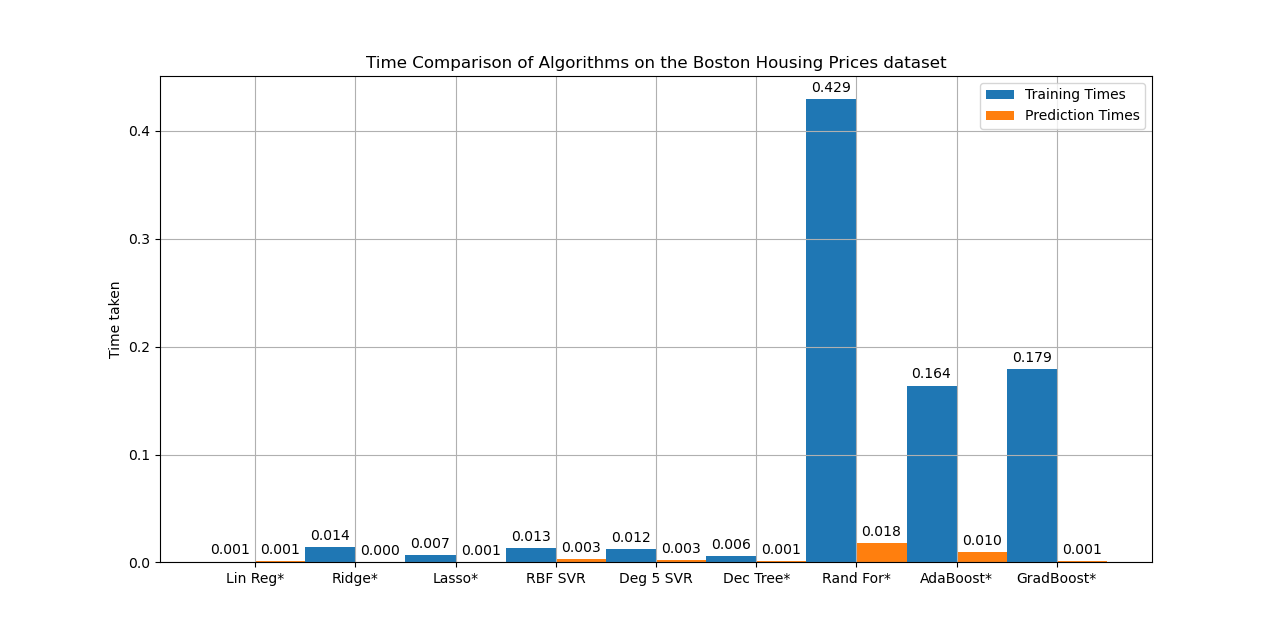
\includegraphics[width=\linewidth]{Images/sup_learn_comp_lin_.png}
  \caption{Linear Y axis}
\end{subfigure}%
\begin{subfigure}{.5\textwidth}
  \centering
  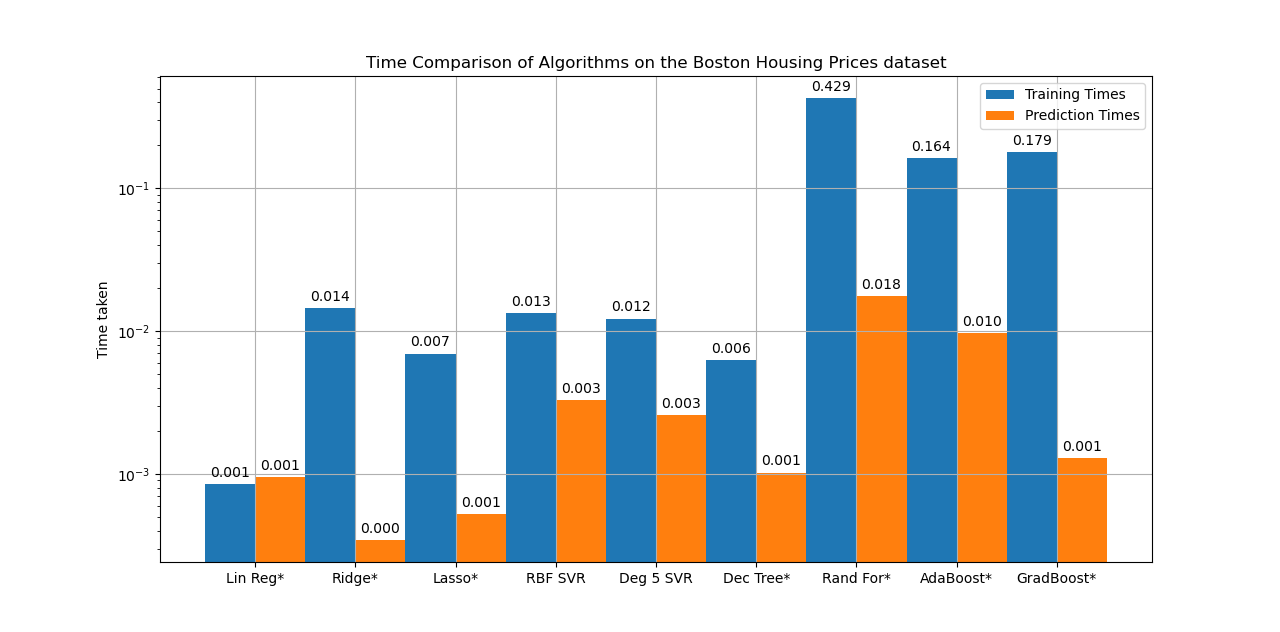
\includegraphics[width=\linewidth]{Images/sup_learn_comp_log_.png}
  \caption{Logarithmic Y axis}
\end{subfigure}
\caption{Comparison of Supervised Learning Regressors}
\end{figure}

SVRs perform abysmally, with the lack of scaling for the input features. The regularized regression models suffer without tuning for its hyper parameters. With direct application the forest and boosting models work best.

\begin{figure}[H]
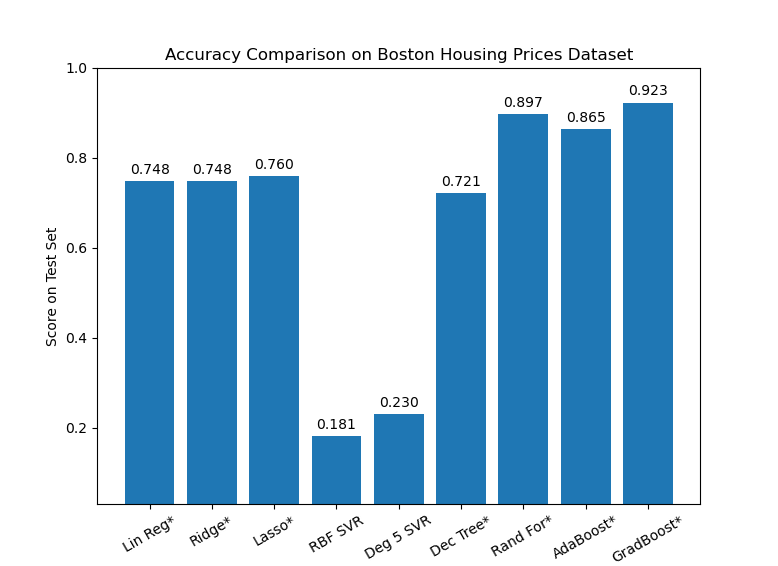
\includegraphics[width=0.6\linewidth]{Images/sup_learn_comp_sco_.png}
\centering
\caption{Score comparison for Supervised Learning Regressors}
\end{figure}


\section{Unsupervised ML Algorithms}

\subsection{Manifold Learning}
Manifold learning is a non linear dimensionality reduction technique. While PCA and other projection based methods are powerful, and provide insights into data, they lack in the preservation of the underlying non linear structure. They are mostly used for visualization, as opposed to transforming train and test sets.

\subsubsection{Locally Linear Embeddings}
LLEs first attempts to find the k-nearest neighbors of every data point and attempts to approximate every data vector as a weighted linear combination of its neighbors. The weights $W_{ij}$ which best reconstruct the point are found.
$$\min E(W) = \sum_{i=1}^N \left\lvert x_i - \sum_{j=1}^k W_{ij}x_j \right\rvert$$
These weights are now used to calculate an embedding vector which will map the coordinates into a lower dimensional space.
$$\min \Phi(Y)\sum_{i=1}^N \left\lvert Y_i - \sum_{j=1}^k W_{ij}Y_j \right\rvert$$
The model needs $\mathcal{O}[D \log(k) N \log(N)]$ for the neighbor finding for $N$ points in $D$ dimensions. The weight matrix construction is the solution of a linear system, $N$ times for every point, and thus takes $\mathcal{O}[DNk^3]$. Finally, a partial eigenvalue decomposition is done, which needs $\mathcal{O}[dN^2]$.

\subsubsection{t-Distributed Stochastic Neighborhood Embedding}
t-SNE converts the affinities of data points into probabilities. t-SNE is however very computationally expensive, as it cross-iterates through the data many times. The algorithm first measures the similarity between the points in the high dimensional space by considering a normal distribution around every point and measuring the density of all points. This gives a probability matrix $P_{ij}$. The size of this distribution can be controlled by the perplexity parameter. This parameter influences the variance of the circle. Now we use a t-distribution with one degree of freedom to map the points, and this gives a set of probabilities which map the points to a lower dimensional space. These are stored in the matrix $Q_{ij}$ The t-distribution is used because of its higher kurtosis, which would help capturing points further away more accurately. We now use KL divergence to measure the difference between the two distributions $P_{ij}$ and $Q_{ij}$, and use gradient descent to make them similar. This divergence loss function we use here does NOT have to be convex, and this can result in different results for every run. For tuning parameters for t-SNE, check out \href{https://distill.pub/2016/misread-tsne/}{this link}.

Here, the toy 'S' dataset is unrolled by these manifold learning methods.
\begin{figure}[H]
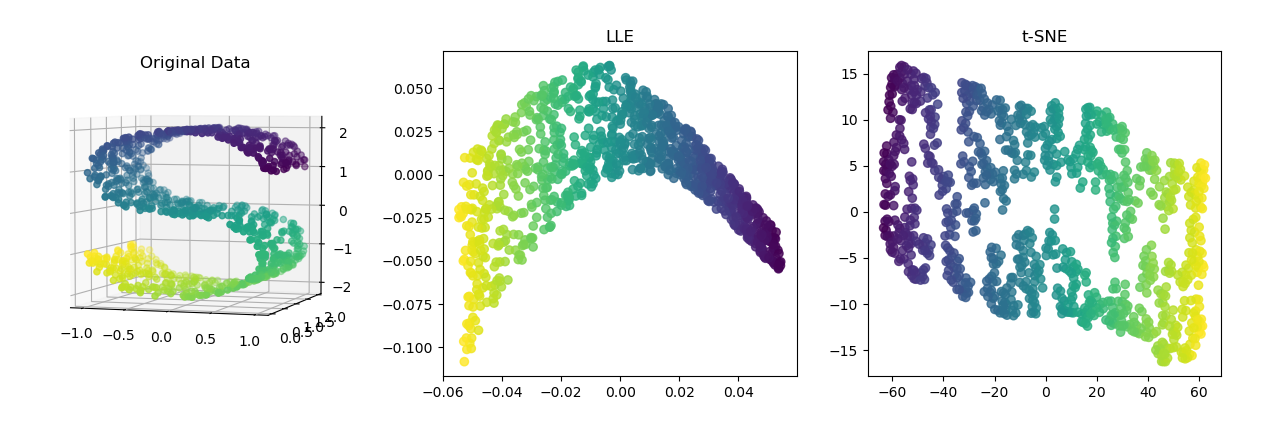
\includegraphics[width=\linewidth]{Images/lle_tsne.png}
\centering
\caption{LLE vs t-SNE}
\end{figure}


\subsection{Gaussian Mixture Models}
A Gaussian mixture model is a probabilistic model which assumes all data points are generated from a mixture of many Gaussian distributions. It uses the expectation-maximization algorithm to find the unknown parameters. First we start with random initialization, and with every step, we set the expected value of the likelihood function as:
$$Q(\theta) = E_{Z|X, \theta}[\log L(\theta; X, Z)]$$
Here, $Z$ is the latent random variable which when observed make likelihood estimation trivial. So now with our guesses, we update the parameters to maximize $Q$.
$$\theta' = \arg \max_{\theta} Q(\theta)$$
These steps are repeated until convergence. This model is really quick and does not bias the mean towards zero, or bias to specific cluster sizes. However, insufficient data may cause it to predict infinite likelihood.

\subsection{Clustering}

Clustering methods are a form of unsupervised learning where the data is reorganized into clusters. Clustering is generally performed for unlabelled data, and hence only a fit method is used on the data. The clustering algorithms in scikit-learn are all in \code{sklearn.cluster}.

\subsubsection{K-Means Clustering}
K-Means can be seen as a special case of Gaussian mixture models. The k-means algorithm divides a set of $N$ samples into $K$ disjoint clusters $C$. Every cluster has a mean $\mu$. The algorithm works to choose those clusters and means which minimise the 'inertia':
$$I = \sum_{i=0}^n \min_{\mu \in C} ||x_i - \mu||^2$$
Inertia can be recognized as a measure of how internally coherent clusters are. Inertia is not a normalized metric, and the smaller the inertia the better. Euclidean distances get inflated in higher dimension spaces, and PCA can help improve the k-means clustering. Euclidean distance also means the model assumes all clusters in the data are roughly spherical, which is obviously not the case everywhere.
Algorithmically, the model aims to repeat two steps. The first step assigns each sample to its nearest centroid. The second step creates new centroids by taking the mean value of all of the samples assigned to each previous centroid. The difference between the old and the new centroids are computed and the algorithm repeats these last two steps until this value is less than a threshold. Mini batches can be used to speed up the k-means algorithm computationally.

\subsubsection{Spectral Clustering}
Spectral clustering offers a graph theoretical approach to clustering. It considers all the data points to be nodes of a graph. We construct our graph with a k-nearest neighbours algorithm. We first find the degree matrix and adjacency matrix of the graph. The degree matrix is a diagonal matrix where the value at entry $(i, i)$ is the degree of node $i$. In an adjacency matrix the row and column indices represent the nodes, and the entries represent the absence or presence of an edge between the nodes. The graph Laplacian is now found, which is simply found by subtracting the adjacency matrix from the degree matrix. We now find the eigenvalues for this matrix. The sorted eigenvalues for the graph Laplacian always has a 0 because we have one connected component - the whole graph. The next eigenvalue is the spectral gap, which tells about the density of the connections. It would be $n$ if there were $n$ data points fully connected to each other, and $0$ if there were none. We now consider the eigenvector corresponding to the spectral gap and progress down the list of its elements. The elements which have a large difference in adjacent values indicate a large gap to cross. Hence, this gap is the clue to the number of clusters in the data. This can be used to pull out different clusters in the data.

\subsubsection{DBSCAN}
Density-based spatial clustering of applications with noise or simply DBSCAN is another clustering algorithm. It views clusters as high density islands surrounded in a sea of low density. This allows DBSCAN heavy flexibility in shapes of clusters. The algorithm has two parameters, minimum samples and eps.  A core sample is defined as a sample in the dataset such that there exist $p$ minimum samples within a distance of eps from it, which are defined as neighbors of the core sample. By definition, any core sample is part of a cluster. The eps parameter must be carefully chosen. When too large, it can return the entire dataset as one cluster, and when too small, it can classify all points as noise.

Here, we can see how these unsupervised clustering models work. The k-means algorithm's central choices for the clusters can easily be spotted in the tips of the moons and the region between the concentric circles. Spectral clustering and DBSCAN perform well. DBSCAN automatically manages to capture the third blob in the fourth row of the data. The other models had to be retrained with different parameters to capture the third cluster in the results of the last row.

\begin{figure}[H]
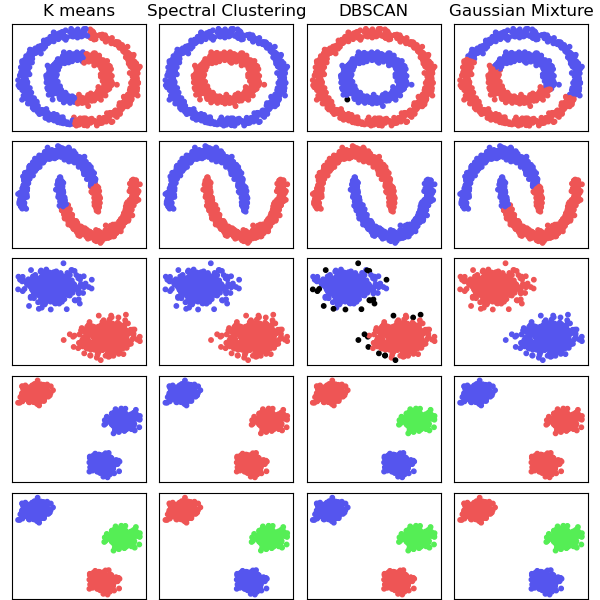
\includegraphics[width=0.9\linewidth]{Images/cluster.png}
\centering
\caption{Clustering Algorithms}
\end{figure}

\subsection{Decomposition}
Most decomposing algorithms are also matrix factorization algorithms. Algorithms of this kind strive to simplify a problem by breaking into simpler subproblems in a divide-and-conquer approach of sorts. The algorithms in this subsection mainly deal with reducing dimensionality by finding the key components in the presented dataset.

\subsubsection{Kernelized PCA}
PCA was already covered in section 2.5, under preprocessing. Kernelized PCA is a modification of vanilla PCA to use kernels to achieve non-linear dimensionality reduction. The kernel is very similar to the methods used in kernelized SVMs. It helps in making the data linearly separable. With linear PCA, the points are still linearly inseparable in the feature space, but when we apply a kernel, we can separate it with fewer components. 

\begin{figure}[H]
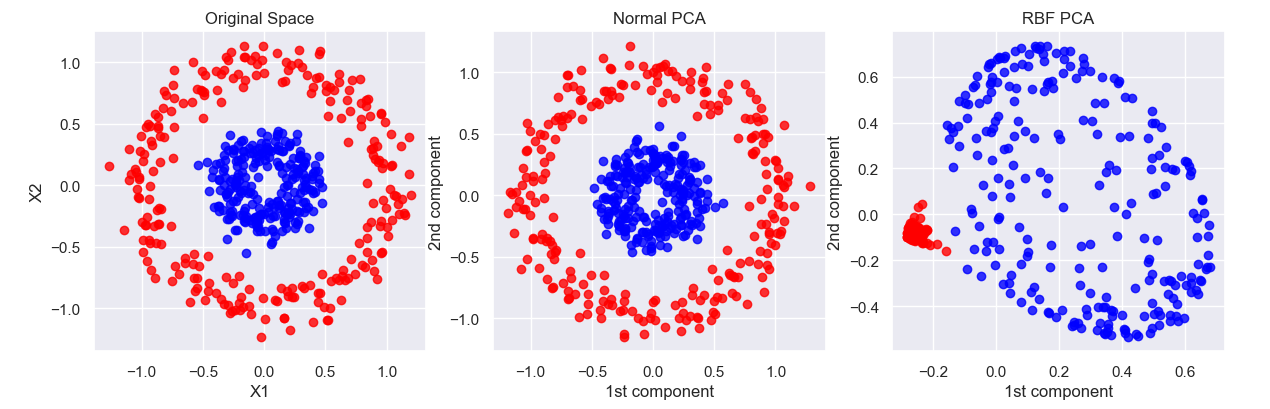
\includegraphics[width=0.9\linewidth]{Images/kernel_pca.png}
\centering
\caption{PCA vs Kernelized PCA}
\end{figure}

\subsubsection{Non-negative Matrix Factorization}
In PCA, the aim was to find orthogonal components which explained most of the variance in the data. In NMF, we use non-negative components and coefficients. The original data is of the form of a matrix $X$, and NMF finds two smaller matrices $W$ and $H$ such that $X \simeq X' = WH$. The squared Frobenius norm is used to evaluate the difference between the matrices, which is then minimised to get a matrix as close as possible to the original.
$$L = \frac{1}{2} ||X-X'||^2 = \frac{1}{2} \sum_{i, j} (X_{i, j} - X'_{i, j})^2$$
NMF can be used in place of PCA and its variants when the data matrix does not have negative values. As with elastic net, we can also add a generalised $L_1$ norm for the data matrix to induce a regularization effect on the data. Other measures of distance such as the KL divergence can also be used. NMF algorithm uses two steps - coordinate descent which estimates the two smaller matrices, and then a multiplicative update which updates the product to calculate new loss. The storage of the result can be done in a sparse array, and the results can be better interpreted due to the absence of negative signs.

Here, we have two signals, a y-shifted sine wave, and a y-shifted digital wave. They were interspersed with random noise and put into a matrix. Now, the NMF algorithm was told there were 2, 3 and 4 components respectively in the data. The random noise does manage to confuse the algorithm in the 2 component part, but the algorithm separates 3 components exactly, and the 4th and higher components are 0. The noise component does steal some gain from the digital component and the sine.

\begin{figure}[H]
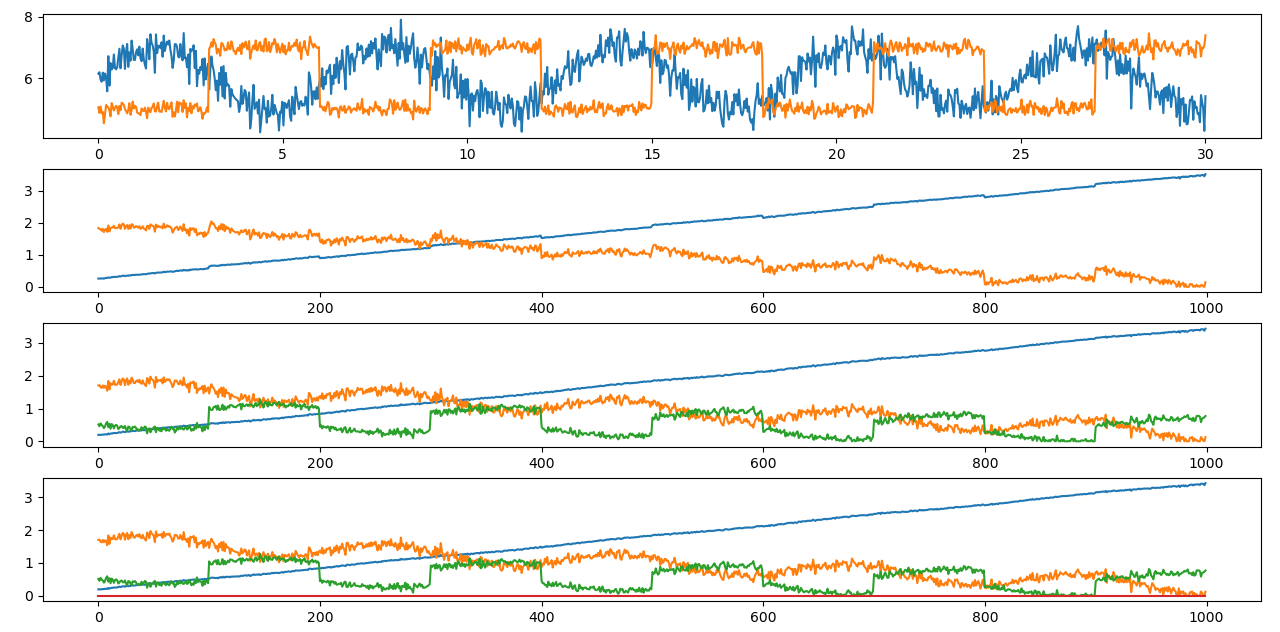
\includegraphics[width=\linewidth]{Images/nmf.png}
\centering
\caption{NMF on signals}
\end{figure}


\end{document}